%%% The main file. It contains definitions of basic parameters and includes all other parts.

%% Settings for single-side (simplex) printing
% Margins: left 40mm, right 25mm, top and bottom 25mm
% (but beware, LaTeX adds 1in implicitly)
\documentclass[12pt,a4paper]{report}
\setlength\textwidth{145mm}
\setlength\textheight{247mm}
\setlength\oddsidemargin{15mm}
\setlength\evensidemargin{15mm}
\setlength\topmargin{0mm}
\setlength\headsep{0mm}
\setlength\headheight{0mm}
% \openright makes the following text appear on a right-hand page
\let\openright=\clearpage

%% Settings for two-sided (duplex) printing
% \documentclass[12pt,a4paper,twoside,openright]{report}
% \setlength\textwidth{145mm}
% \setlength\textheight{247mm}
% \setlength\oddsidemargin{14.2mm}
% \setlength\evensidemargin{0mm}
% \setlength\topmargin{0mm}
% \setlength\headsep{0mm}
% \setlength\headheight{0mm}
% \let\openright=\cleardoublepage

%% Generate PDF/A-2u
\usepackage[a-2u]{pdfx}

%% Character encoding: usually latin2, cp1250 or utf8:
\usepackage[utf8]{inputenc}

%% Prefer Latin Modern fonts
\usepackage{lmodern}

%% Further useful packages (included in most LaTeX distributions)
\usepackage{amsmath}        % extensions for typesetting of math
\usepackage{amsfonts}       % math fonts
\usepackage{amsthm}         % theorems, definitions, etc.
\usepackage{bbding}         % various symbols (squares, asterisks, scissors, ...)
\usepackage{bm}             % boldface symbols (\bm)
\usepackage{graphicx}       % embedding of pictures
\usepackage{fancyvrb}       % improved verbatim environment
\usepackage{natbib}         % citation style AUTHOR (YEAR), or AUTHOR [NUMBER]
\usepackage{subcaption}     % include subfigures
\usepackage[nottoc]{tocbibind} % makes sure that bibliography and the lists
			    % of figures/tables are included in the table
			    % of contents
\usepackage{dcolumn}        % improved alignment of table columns
\usepackage{booktabs}       % improved horizontal lines in tables
\usepackage{paralist}       % improved enumerate and itemize
\usepackage{xcolor}         % typesetting in color
\usepackage[inline]{enumitem} % inline enumeration
\usepackage{multirow}
\usepackage{adjustbox}      % adjust table's width to pagewidth
\usepackage{subcaption}     % Tabulars above each other, subfigures
\usepackage{caption}        % subfigures
\usepackage{listings}       % for code snippets

%%% Package setup

\definecolor{constants}{rgb}{0.8705882352941177, 0.5607843137254902, 0.0196078431372549}
\definecolor{functions}{rgb}{0.00392156862745098, 0.45098039215686275, 0.6980392156862745}
\definecolor{symbols}{rgb}{0.8352941176470589, 0.3686274509803922, 0.0}
\definecolor{background}{rgb}{0.9434690698074405, 0.9435003180635085, 0.9433778365501777}
\definecolor{keywords}{rgb}{0.8, 0.47058823529411764, 0.7372549019607844}
\definecolor{types}{rgb}{0.33725490196078434, 0.7058823529411765, 0.9137254901960784}
\definecolor{comments}{rgb}{0.00784313725490196, 0.6196078431372549, 0.45098039215686275}

\lstset{
  language=Python,
  basicstyle={\footnotesize\ttfamily},
%  backgroundcolor=\color{background},
  escapechar=@,
  commentstyle=\color{comments},
  keywordstyle=\color{keywords},
  numbers=none,
  breaklines=true,
  breakatwhitespace=true,
  tabsize=2,
  captionpos=b,
  float,
}




%%% Basic information on the thesis

% Thesis title in English (exactly as in the formal assignment)
\def\ThesisTitle{Document embedding using Transformers}

% Author of the thesis
\def\ThesisAuthor{David Burian}

% Year when the thesis is submitted
\def\YearSubmitted{2023}

% Name of the department or institute, where the work was officially assigned
% (according to the Organizational Structure of MFF UK in English,
% or a full name of a department outside MFF)
\def\Department{Institute of Formal and Applied Linguistics}

% Is it a department (katedra), or an institute (ústav)?
\def\DeptType{Institute}

% Thesis supervisor: name, surname and titles
\def\Supervisor{Jindřich, Libovický Mgr. Ph.D.}

% Supervisor's department (again according to Organizational structure of MFF)
\def\SupervisorsDepartment{Institute of Formal and Applied Linguistics}

% Study programme and specialization
\def\StudyProgramme{Computer Science}
\def\StudyBranch{Artificial Intelligence}

% An optional dedication: you can thank whomever you wish (your supervisor,
% consultant, a person who lent the software, etc.)
\def\Dedication{%
Dedication.
}

% Abstract (recommended length around 80-200 words; this is not a copy of your thesis assignment!)
\def\Abstract{%
Abstract.
}

% 3 to 5 keywords (recommended), each enclosed in curly braces
\def\Keywords{%
  {text embedding} {document embedding} {transformers} {document
  classification} {document similarity}
}

%% The hyperref package for clickable links in PDF and also for storing
%% metadata to PDF (including the table of contents).
%% Most settings are pre-set by the pdfx package.
\hypersetup{unicode}
\hypersetup{breaklinks=true}

% Definitions of macros (see description inside)
%%% This file contains definitions of various useful macros and environments %%%
%%% Please add more macros here instead of cluttering other files with them. %%%

%%% Minor tweaks of style

% These macros employ a little dirty trick to convince LaTeX to typeset
% chapter headings sanely, without lots of empty space above them.
% Feel free to ignore.
\makeatletter
\def\@makechapterhead#1{
  {\parindent \z@ \raggedright \normalfont
   \Huge\bfseries \thechapter. #1
   \par\nobreak
   \vskip 20\p@
}}
\def\@makeschapterhead#1{
  {\parindent \z@ \raggedright \normalfont
   \Huge\bfseries #1
   \par\nobreak
   \vskip 20\p@
}}
\makeatother

% This macro defines a chapter, which is not numbered, but is included
% in the table of contents.
\def\chapwithtoc#1{
\chapter*{#1}
\addcontentsline{toc}{chapter}{#1}
}

% Draw black "slugs" whenever a line overflows, so that we can spot it easily.
\overfullrule=1mm

%%% Macros for definitions, theorems, claims, examples, ... (requires amsthm package)

\theoremstyle{plain}
\newtheorem{thm}{Theorem}
\newtheorem{lemma}[thm]{Lemma}
\newtheorem{claim}[thm]{Claim}

\theoremstyle{plain}
\newtheorem{defn}{Definition}

\newtheorem{repre_prop}{Property}

\theoremstyle{remark}
\newtheorem*{cor}{Corollary}
\newtheorem*{rem}{Remark}
\newtheorem*{example}{Example}

%%% An environment for proofs

\newenvironment{myproof}{
  \par\medskip\noindent
  \textit{Proof}.
}{
\newline
\rightline{$\qedsymbol$}
}

%%% An environment for typesetting of program code and input/output
%%% of programs. (Requires the fancyvrb package -- fancy verbatim.)

\DefineVerbatimEnvironment{code}{Verbatim}{fontsize=\small, frame=single}

%%% The field of all real and natural numbers
\newcommand{\R}{\mathbb{R}}
\newcommand{\N}{\mathbb{N}}

%%% Useful operators for statistics and probability
\DeclareMathOperator{\pr}{\textsf{P}}
\DeclareMathOperator{\E}{\textsf{E}\,}
\DeclareMathOperator{\var}{\textrm{var}}
\DeclareMathOperator{\sd}{\textrm{sd}}

%%% Transposition of a vector/matrix
\newcommand{\T}[1]{#1^\top}

%%% Various math goodies
\newcommand{\goto}{\rightarrow}
\newcommand{\gotop}{\stackrel{P}{\longrightarrow}}
\newcommand{\maon}[1]{o(n^{#1})}
\newcommand{\abs}[1]{\left|{#1}\right|}
\newcommand{\dint}{\int_0^\tau\!\!\int_0^\tau}
\newcommand{\isqr}[1]{\frac{1}{\sqrt{#1}}}
\DeclareMathOperator*{\argmin}{\arg\!\min\medspace}
\DeclareMathOperator*{\argmax}{\arg\!\max\medspace}

%%% Various table goodies
\newcommand{\pulrad}[1]{\raisebox{1.5ex}[0pt]{#1}}
\newcommand{\mc}[1]{\multicolumn{1}{c}{#1}}


% Title page and various mandatory informational pages
\begin{document}
%%% Title page of the thesis and other mandatory pages

%%% Title page of the thesis

\pagestyle{empty}
\hypersetup{pageanchor=false}
\begin{center}

\centerline{\mbox{
\includegraphics[width=166mm]{./img/logo-en.pdf}}}

\vspace{-8mm}
\vfill

{\bf\Large MASTER THESIS}

\vfill

{\LARGE\ThesisAuthor}

\vspace{15mm}

{\LARGE\bfseries\ThesisTitle}

\vfill

\Department

\vfill

{
\centerline{\vbox{\halign{\hbox to 0.45\hsize{\hfil #}&\hskip 0.5em\parbox[t]{0.45\hsize}{\raggedright #}\cr
Supervisor of the master thesis:&\Supervisor \cr
\noalign{\vspace{2mm}}
Study programme:&\StudyProgramme \cr
\noalign{\vspace{2mm}}
Study branch:&\StudyBranch \cr
}}}}

\vfill

% Zde doplňte rok
Prague \YearSubmitted

\end{center}

\newpage

%%% Here should be a bound sheet included -- a signed copy of the "master
%%% thesis assignment". This assignment is NOT a part of the electronic
%%% version of the thesis. DO NOT SCAN.

%%% A page with a solemn declaration to the master thesis

\openright
\hypersetup{pageanchor=true}
\pagestyle{plain}
\pagenumbering{roman}
\vglue 0pt plus 1fill

\noindent
I declare that I carried out this master thesis independently, and only with the cited
sources, literature and other professional sources. It has not been used to obtain another
or the same degree.

\medskip\noindent
I understand that my work relates to the rights and obligations under the Act No.~121/2000 Sb.,
the Copyright Act, as amended, in particular the fact that the Charles
University has the right to conclude a license agreement on the use of this
work as a school work pursuant to Section 60 subsection 1 of the Copyright~Act.

\vspace{10mm}

\hbox{\hbox to 0.5\hsize{%
In \hbox to 6em{\dotfill} date \hbox to 6em{\dotfill}
\hss}\hbox to 0.5\hsize{\dotfill\quad}}
\smallskip
\hbox{\hbox to 0.5\hsize{}\hbox to 0.5\hsize{\hfil Author's signature\hfil}}

\vspace{20mm}
\newpage

%%% Dedication

\openright

\noindent
\Dedication

\newpage

%%% Mandatory information page of the thesis

\openright

\vbox to 0.5\vsize{
\setlength\parindent{0mm}
\setlength\parskip{5mm}

Title:
\ThesisTitle

Author:
\ThesisAuthor

\DeptType:
\Department

Supervisor:
\Supervisor, \SupervisorsDepartment

Abstract:
\Abstract

Keywords:
\Keywords

\vss}

\newpage

\openright
\pagestyle{plain}
\pagenumbering{arabic}
\setcounter{page}{1}


%%% A page with an automatically generated table of contents of the master thesis

\tableofcontents

%%% Each chapter is kept in a separate file
\chapter*{Introduction}
\addcontentsline{toc}{chapter}{Introduction}



\chapter{Document representation}\label{chapter:document_representation}

We dedicate this chapter to the center point of our thesis --
representing documents with vectors. The goal of this chapter is to define the
desired qualities of our embeddings and illustrate them on examples.

\section{Desirable qualities of document representations}

Since there are many ways how to embed a document we deemed it necessary to
describe what are the target qualities of the embeddings. There are two
dimensions along which we asses document representations: \emph{depth} and
\emph{breadth}. \emph{Depth} dimension defines how deep is the model's
understanding of the input text. \emph{Breadth} dimension defines the amount of
information the model is able to process. These dimensions are in a sense
contradictory to each other. We cannot expect a fully learned model of a fixed
size to deepen its understanding of the input while maintaining the same
maximum input size. Thus we are searching for a ideal ratio of these two
qualities.

\subsection{Text understanding}

In the depth dimension we study how well the model understands its input. For
an input \emph{``This is a really nimble horse. You should be cautious when
riding him.''} we would like the model to understand that \emph{``him''} refers to
the \emph{``nimble horse''}. Or that the meaning of \emph{``stick''} in the
following sentences is largely different:

\begin{itemize}
  \item \emph{``You are really good at tennis. You should stick to it.''}
  \item \emph{``Some dogs really like to fetch a stick, some just carry it.''}
\end{itemize}

To produce embedding that would reliably reflect the input's meaning, we expect
the model to see the words in context of their relationship to other words. To
do so, architectures that enable deep text understanding allow the model to
compute with relationships of ordered subwords, words or sequences of words.
Such architectures are able to put each word in relevant context and thus
recover all the meanings of each sequence of words if they are given enough
training data.

To compute with relationships of ordered subwords, the neural network must
connect representations of two subwords such that the connections also carry
the information about the subwords' ordering. The same holds for computing with
relationships of ordered words or sequences of words.

To give some examples we can pick some representative embedding models along
the depth dimension going from the ones that show the shallowest understanding
of their input to those who show the deepest. At the beginning, there are
models that ignore both word ordering and their relationships. An example of
such model is TF-IDF. If we go deeper we run into Paragraph
Vector~\cite{le2014distributed}, that takes word relationships into an account,
but ignores word ordering to a certain degree. Next there are models with
architectures based on one-directional or two-directional RNNs. These models
compute with ordering of words implicitly, but do not have the capacity to
consider some word relationships directly. Finally there are models that are
based on the architecture of Transformer~\cite{vaswani2017attention}. Such
models not only take the word ordering into consideration, but are also able to
compute over all relationships between input's text units. An example of such
architecture is SBERT~\cite{reimers2019sentence}, which is essentially an
instance of BERT~\cite{devlin2019bert} finetuned on NLI datasets to encourage
deeper text understanding.

\subsection{Maximum input length}

In the breadth dimension we study the maximum context length of the model. Put
simply, we study the maximum number of tokens the model is able to process. The
longer the maximum context length is, the longer text we can coherently embed.

Model's context length is especially important when we expect the properties of
the piece of text to vary throughout it. For such texts the embedding of its
beginning would be different than the embedding of its end or of the whole
text. Comparing embeddings of long texts, thus requires to consider the text as
a whole and embed it with a model whose maximum context is larger or equal than
the given text's length.

If we revisit the models mentioned in the previous section, we realise the
order of the mentioned models flips. The models with the smallest maximum
context are Transformers with classical attention mechanisms. They are
typically not limited by their architecture, but by the memory they consume for
longer inputs. The large memory consumption originates in the classical
attention mechanism, which takes into account all of the $n^2$ relationships
among the $n$ input tokens. Though recently there have been many improvements
to the implementation of classical attention(TODO: ref) which improves their
efficiency, and there are other attention mechanisms which offer more efficient
alternative, Transformers are nevertheless costly for longer inputs both in
terms of memory and time. Next type of models are those built using RNNs.
Though RNNs can in theory process unlimited number of tokens, in practice they
are known for ``forgetting'' past tokens, once the input is long enough (TODO:
ref). On the other hand, Paragraph Vector or TF-IDF can both process in theory
limitless number of words. In practice Paragraph Vector is limited by the
dimension of the document embedding, which can be, however, scaled arbitrarily.

\subsection{Combining depth and breadth}

As we have hinted above, the goal of this thesis is to combine deep
understanding with longer maximum contexts. Combination of both qualities would
result in a model that can not only register and compute with relationships of
words, but do so over large gaps of unrelated tokens. For example, in \emph{``I
really like your T-shirt. It almost looks as if it was designed by some really
alternative guy living in some cave in Gran Canaria. You should definitely wear
it more often.''}, we would expect such model to connect \emph{``it''}
in the last sentence with the \emph{``T-shirt''} from the first sentence.

To find a compromise, we combine models of the two extremes: models like
Transformer that can understand the input very well and models like Paragraph
Vector which can process very long sequences.

%\chapter{Background}

In this chapter we describe model architectures, concepts and training
methodologies our work uses.


\section{Text embedding}

To allow neural networks to process text, each continuous piece of text is
mapped to a series of vectors that represent it. This mapping and its result is
called an embedding. Traditionally we would split the input text
to sub-words and allow the network to change their embedding arbitrarily to
solve some end task. Example of such task is sub-word prediction, where the
network guesses masked-out sub-word.

In our work we train a network to map a long piece of text to a single vector.
As the size of the embedding is limited, we expect the network to effectively
compress the input. In this work our aim is not to reconstruct the input from
the embedding, but rather to capture both the structure and meaning of the text.

\section{Paragraph Vector}

Paragraph Vector~\cite{le2014distributed} (also known as Doc2Vec) is a
text-embedding model that is an extension of
Word2Vec~\cite{mikolov2013efficient}. Paragraph Vector is composed of two
sub-models called Distributed Memory (or DM) and Distributed Bag of Words (or
DBOW). Both DM and DBOW are trained on token prediction. To predict masked-out
tokens, both models use embedding of the whole input, while DM additionally
computes word embeddings. In practice, each embedded piece of text (a word or
an input) gets an identifier, which is used as an index into an embedding
matrix that stores the vector representations.

Paragraph Vector, thanks to its simplicity, can be trained quickly, even with
limited computational resources. Additionally the model can embed texts of any
length. However, Paragraph Vector has three major disadvantages. First, it
ignores text structure, by assuming the input is a bag of words rather than its
sequence. Second, because it is very simple model, it does not have the
capability to understand complex relationships of words, sentences or
paragraphs. Third, due to how embeddings are computed, the inference time is
very long, since it is necessary to train the model until convergence on the
previously unseen test input.

% TODO: my own graphic here

\begin{figure}[h]
    \centering
    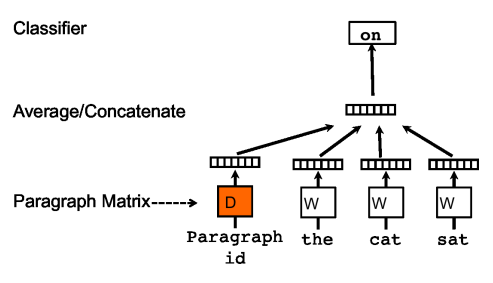
\includegraphics[width=0.4\textwidth]{./img/pv-dm.png}
    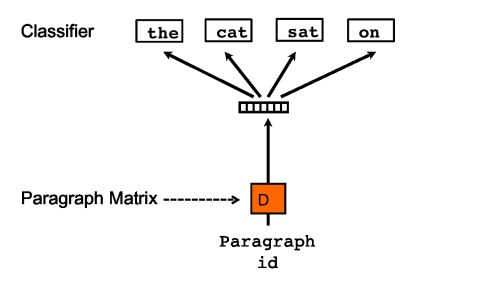
\includegraphics[width=0.4\textwidth]{./img/pv-dbow.png}
    \caption{PV-DM and PV-DBOW architectures.\label{fig:pv-dm_pv-dbow}}
\end{figure}

\section{SBERT}

Sentence-BERT~\cite{reimers2019sentence} (or SBERT) a composition of a
Transformer (TODO: citation) encoder with a pooling layer above its final
hidden states. The model is warm-started from a pre-trained Transformer such as
BERT (TODO: citation), RoBERTa (TODO: citation) or MPNet (TODO: citation). Then
it is fine-tuned on NLI datasets so that the pooled representations of the
whole inputs are comparable using cosine. The goal is that a semantic
difference between two inputs should correspond to the cosine between the
two pooled representations.

Thanks to higher parameter count, SBERT can understand more complex
relationships than Paragraph Vector. As no parameter adjustment is necessary
during inference, SBERT predicts embeddings very quickly which makes it
suitable for search applications. The disadvantage is that it can process text
only up to a certain length and unfortunately the same training cannot be used
for longer texts due to lack of appropriate datasets.

\section{Sparse attention}

Traditional Transformer encoder uses full-attention, which means that every
token can interact (or attend) to any other token. This type of attention
creates quadratic number of interactions to input length and therefore also
quadratic time and space complexity. This seriously limits use of transformers
for longer inputs even with efficient cuda kernels (TODO: really? Citation
needed). To overcome this issue, interactions between some tokens are ignored.
Such type of attention is called sparse.

TODO: My graphic of attentions

\begin{figure}[h]
    \centering
    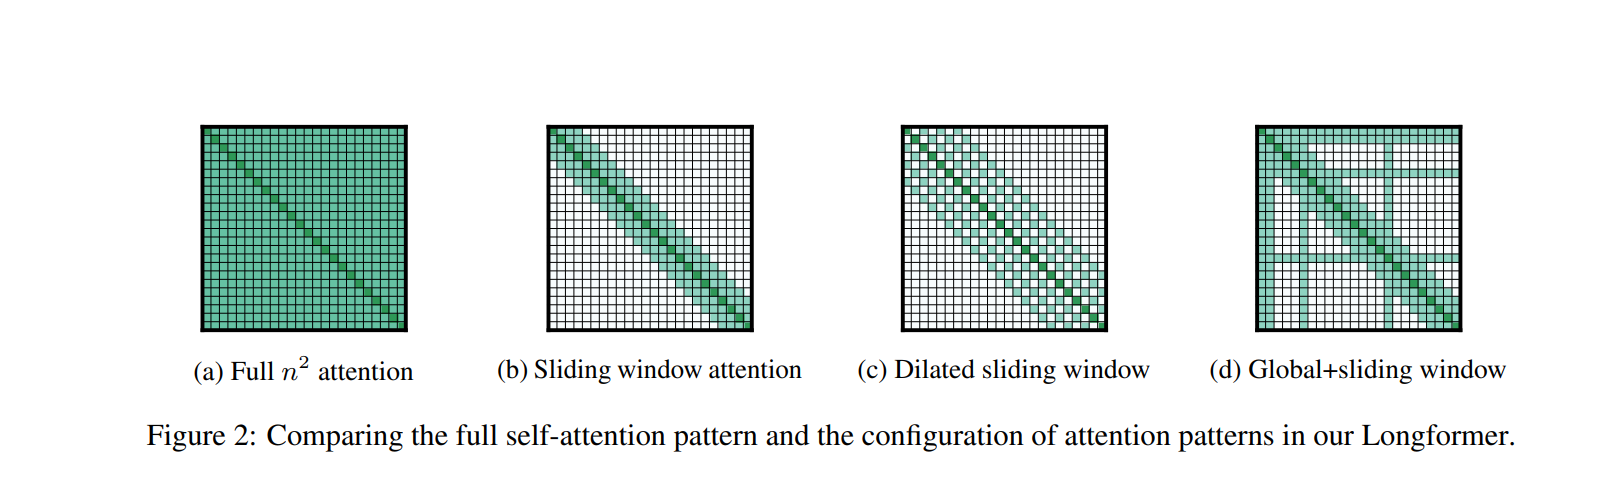
\includegraphics[width=0.9\textwidth]{./img/longformer_attention.png}
    \caption{Longformer attention matrix.\label{fig:longformer_sparse_att}}
\end{figure}

Sparse attention can have different designs but they are usually composed of
several types of mechanisms (such as sliding window, global, random -- I can
write more about this).

\subsection{Longformer}

Longformer~\cite{beltagy2020longformer}, is a transformer with sparse attention
that combines global and sliding window mechanisms. It is warm-started from
RoBERTa weights with its learned embeddings copied 4 times. Thus Longformer can
process inputs up to 4096 tokens long. Then the model was fine-tuned using
Masked Language Modelling (or MLM) on a dataset of long documents such as
Wikipedia articles or books.

There are many others sparse attention models, but we ephasize Longformer since
it is one of the best performing~\cite{tay2020long} and yet has relatively
simple attention mechanism, which makes it a suitable benchmark.

\section{Teacher-student training}

Teacher-student training is a setup in which we train a model (a student)
according to the relationship of its output with outputs of another model (a
teacher), which is frozen. The desired relationship can differ, but often we
aim to minimize the difference between the two outputs to simulate the teacher
model by the student. Teacher-student training can been used to dramatically
decrease the size of a model, while at the same time only slightly decreasing
its performance. Another use of this method is in multi-modal learning when
more modalities of the same input are available. In such cases we can have
several teacher models, each for different modality, providing their outputs to
the loss of a single student model.

TODO: some graphic

\section{Canonical Correlation Analysis}

Canonical Correlation Analysis (CCA) computes linear projections of two vectors
such that their projections are maximally correlated. To define CCA properly,
let us look at its mathematical formulation.

\begin{defn}[Canonical Correlation Analysis]\label{def:cca}

  For two matrices $X_1 \in \mathbb{R}^{n_1 \times m_1}$ and $X_2 \in
  \mathbb{R}^{n_2 \times m_1}$, Canonical Correlation Analysis finds $p \in
  \mathbb{R}^m_1$ and $q \in \mathbb{R}^m_2$ that maximize

  \begin{equation}
    \begin{split}
      & corr(X_1p, X_2q) = \frac{p^TX_1^TX_2q}{||Xp|| ||Yq||} \\
      \text{s.t.}\quad &||X_1p|| = ||X_2q|| = 1 \\
    \end{split}
  \end{equation}


\end{defn}

Definition~\ref{def:cca} suggests that CCA gives only a single number as the
measure of correlation of two matrices. When the dimensions of the input
vectors are large enough, however, often there is a some combination of
features that results in correlation of 1. This would make CCA relatively
useless in context of high-dimensional spaces. To overcome this issue we assume
multiple correlations for several mutually orthogonal projections. Again, let
us look at the mathematical formulation.

\begin{defn}[Canonical Correlation Analysis in more dimensions]\label{def:cca_more_dim}

  For two matrices $X_1 \in \mathbb{R}^{n_1 \times m_1}$ and $X_2 \in
  \mathbb{R}^{n_2 \times m_1}$, Canonical Correlation Analysis in $k$
  dimensions finds $P \in \mathbb{R}^{m_1 \times k}$ and $Q \in \mathbb{R}^{m_2
  \times k}$ that maximize

  \begin{equation}
    \begin{split}
      &\sum_{i = 1}^k corr(X_1P_{*i}, X_2Q_{*i}) \\
      \text{s.t.}\quad &P^TX_1^TX_1P = I_k = Q^TX_2^TX_2Q \\
    \end{split}
  \end{equation}


\end{defn}

If we consider the conditions in Definition~\ref{def:cca_more_dim}, the
resulting value can be easily formulated as $trace(P^TX_1^TX_2Q) =
trace(P^T\Sigma_{X_1X_2}Q)$, where $\Sigma_{X_1X_2}$ is covariance matrix of
$X_1$ and $X_2$.

TODO: analytical solution to pure CCA

\subsection{CCA as a loss}

CCA can be used as a loss in teacher-student training to establish some sort of
correspondence between the teacher's and the student's outputs. When CCA is
maximized the teacher's and the student's outputs are first linearly
transformed, before the correlation is computed. CCA is therefore weaker
requirement than classical correlation.

The problem of using CCA as a loss is that it is defined in the context of the
whole dataset rather than just a minibatch. It is therefore unclear how CCA for
a pair of minibatches of vectors should be computed. Someone (TODO: citation)
found that using large enough batch size is sufficient for the training to
converge.

\subsection{Deep CCA}

Deep CCA (or DCCA) is an extension of CCA that computes projections using
neural networks. As such it is more powerful than plain CCA as it allows for
non-linear projections. To compute DCCA the network has to be trained on the
pairs of vectors with CCA as its loss.

TODO: graphic of architecture

If CCA is weaker condition than just correlation, DCCA is even weaker since
there is no limit to how the projections should look like.

\subsection{Soft CCA}

Soft CCA reformulates CCA and thus allows its straightforward use in the
context of minibatches. With constraints from Definition~\ref{def:cca_more_dim}
taken into account, CCA can be formulated using Forbenious matrix norm:

\begin{align}
  P^\ast, Q^\ast &= \underset{P, Q}{\argmin} ||X_1P - X_2Q||^2_F \\
  &= \underset{P, Q}{\argmin} trace\Big((X_1P - X_2Q)^T(X_1P - X_2Q)\Big) \\
  &= \underset{P, Q}{\argmin} {-2} trace(P^TX_1^TX_2Q) \\
  &= \underset{P, Q}{\argmax} trace(P^TX_1^TX_2Q) \\
  &= \underset{P, Q}{\argmax} \sum_{i = 1}^k corr(X_1P_{*i}, X_2Q_{*i})
\end{align}

So, in essence minimizing CCA is the same as minimizing the difference between
projections, whose features are decorrelated. This is the formulation Soft CCA
builds on. Soft CCA decomposes CCA into to parts:

\begin{itemize}
  \item minimization of the difference between projections

    \begin{equation}
      ||X_1P - X_2Q||^2_F
    \end{equation}

  \item decorrelation of each projection $P$

    \begin{equation}
      \sum_{i \ne j} (P^TX^T_{mini}X_{mini}P)_{ij} = \sum_{i \ne j} \Sigma_{X_{mini}P},
    \end{equation}

    where $X_{mini}$ is batch-normalized minibatch.

\end{itemize}

To bring correlation matrix of the current minibatch $\Sigma_{X_{mini}P}$
closer to the true covariance, the decorrelation part is in fact computed from
a covariance matrix that is increamentally learned.

In this way Soft CCA increamentally decreases CCA through incrementally learned
approximation of the projections' covariances.

\section{Contrastive loss}

Contrastive losses are types of losses which compare several model's outputs to
each other and based on this comparison they compute a value, which can be used
as a loss. Contrastive loss is often used when the model's goal is to
understand and distinguish different inputs. In this setting, we would penalize
the model if the representations of similar inputs are far apart or if the
representations of different inputs are close. Similar inputs are called
positives, whereas distinct inputs are called negatives.

When no supervised information about the similarity of a pair of inputs is
available, we can use in-batch outputs as negatives. Here we automatically
assume that all our inputs are distinct and that the model should distinguish
between all of them.

\chapter{Related Work}

- approaches so far: the `history'

\chapter{Distilling structural and contextual qualities of document
embeddings}\label{chapter:training_method}

In this chapter, we introduce our method of training document embeddings. We
base our approach on teacher-student training, distilling the knowledge of two
embedding models (referred to as \emph{teachers}) into one  \emph{student}
model. Section~\ref{section:training_method} explains our training method in
detail and outlines the used loss function. In the rest of this chapter, we
describe the two teacher models in Section~\ref{section:teacher_models} and the
student in Section~\ref{section:student_model}.

\section{Training methodology}\label{section:training_method}

Our training methodology aims to train an embedding model such that its
embeddings more faithfully represent the input. As we describe in
Chapter~\ref{chapter:document_representation}, we distinguish two qualities of
faithful representations: structural and contextual. The goal is to instill
both qualities into a single embedding model. To do so, we use teacher-student
training with two teacher embedding models, one with high structural capacity
and the other with high contextual capacity.

In the following subsections, we describe teacher-student training in detail
and give a high-level overview of the proposed loss function.

\subsection{Teacher-student training}

In the teacher-student training, we train a student model based on a frozen
teacher model. The goal is to make the student model imitate the teacher model,
thereby digesting the teacher's understanding of the input. Although the
student model is generally not expected to outperform the teacher model,
teacher-student training is still valuable in several situations. For instance,
\cite{sanh2019distilbert} use teacher-student training to make a model smaller
while sacrificing only a fraction of its performance. In another scenario,
\cite{reimers2020making} use teacher-student training to enforce similarity
between models' outputs, thereby giving the student model a powerful training
signal.

We assume two embedding models in our setting: a structural teacher
$\Teacher_S$ and a contextual teacher $\Teacher_C$ with high structural and
contextual capacities, respectively. Teacher-student training allows us to
instill both capacities into a third student model {\Student} while avoiding
the architectural limitations of the teachers. We hypothesize that we can
efficiently direct the two training signals so that they do not push against
each other.


\subsection{Abstract loss formulation}\label{section:abstract_loss}


We instill a quality of a teacher's embedding by simply enforcing a similarity
between the teacher's and student's embedding. Since we have two teachers, we
use two similarities $\Loss_S$, and $\Loss_C$, which compare the student's
embedding $y_\Student$ with the structural teacher's embedding $y_{\Teacher_S}$
and the contextual teacher's embedding $y_{\Teacher_C}$, respectively. We show
a graphical overview of the training architecture in
Figure~\ref{fig:teacher_student_train_arch}.

To regulate the mixture of $\Loss_S$ and $\Loss_C$, we introduce weighting
parameter $\lambda$. In the most general form, we assume $\lambda$ to be
dependent on the input text $x$ since the performance of the teacher models
might vary across different inputs. In particular, we can expect $\lambda$ to
depend on the length of the input since, for shorter inputs, the context
is minimal and, therefore, expendable. Abstract formulation of the loss is
given in Equation~\ref{eq:abstract_loss}. We explore concrete options for
$\Loss_S$, $\Loss_C$ and $\lambda(x)$ in Chapter~\ref{chapter:experiments}.

\begin{equation}\label{eq:abstract_loss}
  \Loss(
    x,
    y_\Student,
    y_{\Teacher_S},
    y_{\Teacher_C},
    \lambda
  ) =
    \lambda(x) \Loss_S(y_\Student, y_{\Teacher_S}) +
            (1 - \lambda(x)) \Loss_C(y_\Student, y_{\Teacher_S})
\end{equation}

The two losses could push against each other and slow down or halt the
training. To avoid that, we choose one of the losses to be more strict while
the other to be more forgiving. In that way, the more forgiving loss should
adapt to the strict one instead of pushing against it. As mentioned in
Section~\ref{section:combine_structural_and_contextual}, we view structural
quality as the more important. Therefore, we choose the structural loss
$\Loss_S$ as the stricter and exact loss, forcing the student to mimic the
structural teacher as much as possible. On the other hand, the contextual loss
$\Loss_C$ should give the student model more freedom in the form of the
produced embedding but still force it to incorporate the information from the
contextual embedding.

\begin{figure}
  \centering
  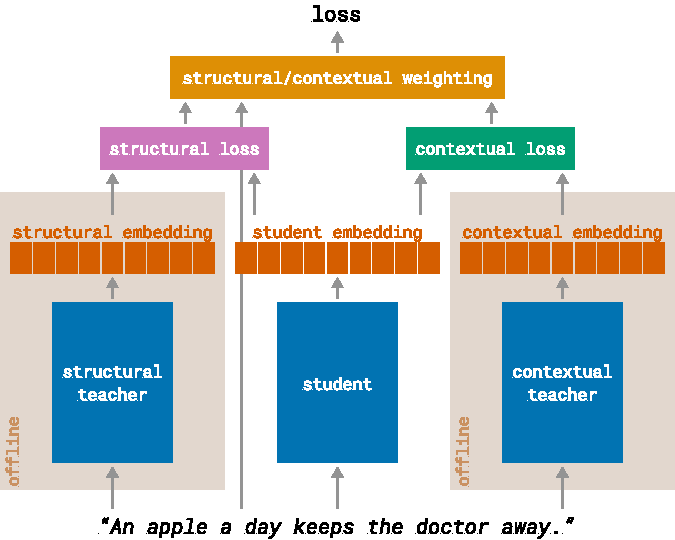
\includegraphics[width=0.8\textwidth]{./img/training_architecture.pdf}

  \caption{The architecture of our teacher-student training. We distill the
  qualities of the teachers' embeddings through corresponding losses into a
  student model. Since we do not update the weights of either teacher,
  the generation of their embeddings can be done offline before training.}

  \label{fig:teacher_student_train_arch}

\end{figure}

\section{Teacher models}\label{section:teacher_models}

This section introduces the teacher models used during our experiments in
Chapter~\ref{chapter:experiments}. We chose Sentence-BERT
\citep{reimers2019sentence} as the structural teacher model and Paragraph
Vector \citep{le2014distributed} (or \emph{PV}) as the context teacher model.
As explained in Chapter~\ref{chapter:document_representation}, each of the two
mentioned models specializes in a different quality of produced embeddings.
SBERT can compare word relationships on many levels and thus understand even
complex text structures. However, it cannot process long texts. On the other
hand, Paragraph Vectors can produce embeddings even for long documents, but they
process text very shallowly, which prohibits understanding any complex
structures. We hope to synthesize both qualities by combining the two
teacher models in a single model.

\subsection{SBERT}

Sentence-BERT is a composition of a BERT-like \citep{devlin2019bert} encoder
with a mean pooling layer above its last layer's hidden states. The model is
finetuned with Natural Language Inference (\emph{NLI}) datasets to produce
semantically meaningful embeddings. We illustrate SBERT's training
architecture in Figure~\ref{fig:sbert}. We have chosen SBERT as a structural
teacher for its high structural capacity and strong performance in
sentence-level text-understanding tasks \citep{reimers2019sentence}.

\begin{figure}
  \centering
  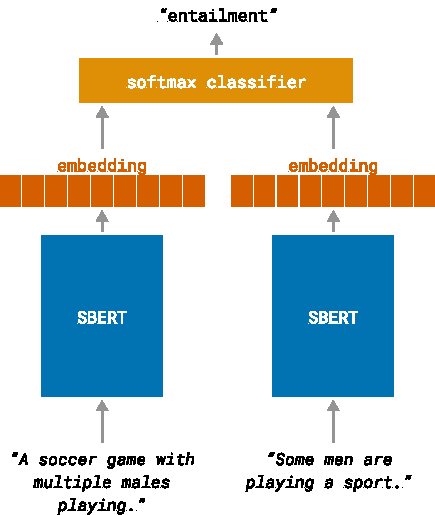
\includegraphics[width=0.5\textwidth]{./img/sbert_architecture.pdf}

  \caption{Siamese network architecture used to train SBERT. The pair of
  sentences from an NLI dataset is classified into three classes
  ``entailment'', ``neutral'' and ``contradiction''.}

  \label{fig:sbert}

\end{figure}

\subsection{Paragraph Vector}\label{section:paragraph_vector}

Paragraph Vector \citep{le2014distributed}, sometimes referred to as Doc2Vec, is a simple
text-embedding model that views the input as a Bag of Words (or BoW). Paragraph
Vector comprises two sub-models: Distributed Memory (DM) and Distributed Bag of
Words (DBOW). While each model is trained separately, the authors recommend combining both architectures into a single model, where the combined models' embeddings are simply concatenated. The models are trained to
predict a word within a window in the given document. As shown in
Figure~\ref{fig:dbow}, DBOW bases its prediction only on the whole paragraph's embedding. On the other hand, DM, whose architecture is depicted in
Figure~\ref{fig:dm}, additionally uses the embeddings of the surrounding words
within a given window.

We chose Paragraph Vector as a contextual teacher due to its unique
architecture, which forces the model to develop a single vector that summarizes
the common theme of the document. Moreover, Paragraph Vector does not have a
limited maximum input length, so as a contextual teacher, it will always
provide some signal to the student regarding the document's context. Also, even
though Paragraph Vector cannot match the performance of substantially more
complex models such as Transformers, \cite{dai2015document} show that for
larger datasets, Paragraph Vector, outperforms classical embedding models such
as Latent Dirichlet Allocation \citep{blei2003latent} or TF-IDF weighted BoW
model \citep{harris1954distributional}. Finally, Paragraph Vector's simple
architecture allows it to train on significantly larger text corpora than other
bigger models, such as SBERT. Therefore, for a given computational budget,
Paragraph Vector would see more documents during training than SBERT, which may
give it a slight advantage.

\begin{figure}
  \centering
  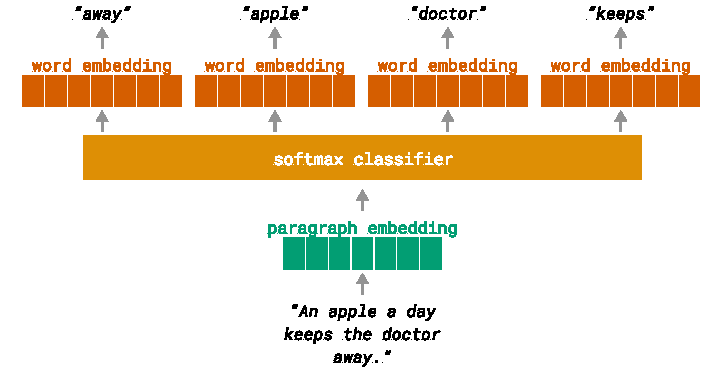
\includegraphics[width=0.8\textwidth]{./img/dbow_architecture.pdf}

  \caption{Architecture of Distributed Bag of Words. The model predicts words
  from a document, only using the document's embedding.}

  \label{fig:dbow}
\end{figure}

\begin{figure}
  \centering
  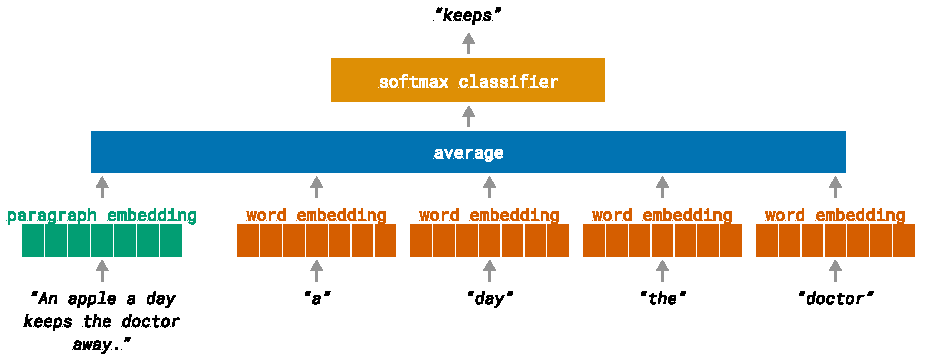
\includegraphics[width=1\textwidth]{./img/dm_architecture.pdf}

  \caption{Distributed Memory model architecture. The model predicts the input
  words' neighboring word for the input paragraph.}

  \label{fig:dm}

\end{figure}

\section{Student model}\label{section:student_model}

In our teacher-student training, the student model is our primary embedding
model, which we train based on the outputs of the teacher models. By using
teacher-student training, we can avoid some of the architectural drawbacks of
both teacher models while still benefiting from the qualities of the teachers'
embeddings. We choose the student's architecture at a midpoint between
the two teachers' architectures. In other words, not to be as complex as the
architecture of SBERT, so it can process longer inputs while still having a
manageable memory footprint, but not as simple as the architecture of PV, so
that the student can model complex world relationships. We chose a Transformer
with a sparse attention mechanism. Transformer is a well-tested architecture
that is used throughout NLP. Additionally, with sparse attention, Transformers
consume a relatively small amount of memory even for longer inputs, as we
explain in Section~\ref{section:efficient_self_attn}. Another consideration is
that we need a pre-trained model, as our method is not suited to train a model
from scratch but to finetune a model's document embeddings.

Contrary to the selection of architecture, selecting a concrete model is not
crucial to our method. Our choice of the concrete model is governed more by
practical considerations rather than the conditions of our method. Since we
have limited computational resources, we prefer a smaller model that we can fit
on a consumer-grade GPU card. We also value the model's performance, ease of
use, and simplicity. We choose Longformer \citep{beltagy2020longformer} as it
is reasonably small, memory efficient, performs above average compared to other
similar models \citep{tay2020long}, and its self-attention mechanism is
straightforward. Other alternatives are BigBird \citep{zaheer2020big}, or if we
would not mind a more complex model, we could use Reformer
\citep{kitaev2020reformer}, Linformer \citep{wang2020linformer} or Performer
\citep{choromanski2020rethinking}.

\subsection{Longformer}

Longformer \citep{beltagy2020longformer} is a Transformer encoder with sparse
attention. Because we refer to Longformer's configuration and training in the
following chapters, we briefly explain Longformer's self-attention mechanism
and the training data of the pre-trained checkpoint.


\subsubsection{Self-attention mechanism}

Longformer has a sparse self-attention mechanism that composes three different
patterns: local, global, and dilated local attention. Local attention is simply
full attention but only within the neighborhood of $\frac{1}{2}\omega$ tokens
on either side of the key token. $\omega$ can be set differently per
self-attention layer. In global attention, few selected tokens attend to all
other tokens. The tokens on which Longformer computes global attention can be
selected per each input. Global attention's parameters are not pre-trained.
Instead, at the beginning of the training, they are initialized by the
parameters from local attention and finetuned for a given task. With dilated
local attention, every key token attends to every $k$ neighboring query token.
So, it is analogous to a one-dimensional Convolution layer
\citep{van2016wavenet} with stride, or dilatation of $k$. However, to use
dilated local attention, one has to use a custom CUDA kernel or a slow
implementation in Python using loops. The authors also provide a reasonably
fast, memory-efficient block implementation for global and local
attention.

\subsubsection{Training}

Longformer is warm-started from a RoBERTa \citep{liu2019roberta} checkpoint
with its learned positional embeddings duplicated eight times to support inputs
up to 4096 tokens long. The authors show that duplicating RoBERTa's positional
embeddings is faster than training position embeddings for all 4096 positions
from scratch. Then, the authors train Longformer using MLM on long documents
for 65k gradient steps to improve its capabilities for longer inputs. The
training corpus overlaps with RoBERTa's pretraining corpus but is more focused
on longer pieces of text. It includes the following datasets:

\begin{itemize}

  \item Book corpus \citep{zhu2015aligning}

  \item English Wikipedia

  \item One-third of articles from Realnews dataset \citep{zellers2019defending}
      with more than 1200 tokens

  \item One-third of the Stories corpus \citep{trinh2018simple}

\end{itemize}

Unfortunately, as of this writing, the Book corpus is unavailable due to
licensing issues. Moreover, we have not been able to find a comparable
alternative. The Stories corpus is also unavailable. However, there is an
alternative\footnote{\url{https://huggingface.co/datasets/spacemanidol/cc-stories}}
that tries to mimic the dataset from the original paper.

\chapter{Experiments}\label{chapter:experiments}

In this chapter, we study and experiment with the training method we introduced
in Chapter~\ref{chapter:training_method}. While the main goal is to outperform
both teacher models and the base student checkpoint, we also want to show that
each teacher contributes to the student's performance.

This chapter is laid out as follows. We describe the training data in
Section~\ref{section:val_training_data}. Next, we discuss how we compare models
in Section~\ref{section:validation_tasks} and present the student's
configuration and define the baselines in
Section~\ref{section:student_model_config_baselines}. Then, we experiment with
the structural loss in Section~\ref{section:structural_loss}. With the
structural loss already given, we find the best performing contextual loss and
the weighting of the two losses in Section~\ref{section:structural_and_contextual}.
Finally, we summarize our experiments and findings in
Section~\ref{section:experiments_summary}.

\section{Training data}\label{section:val_training_data}

We create the training dataset for our validation, labeled as
\Dataset{val-500k}, similarly to how we put together the final training
dataset \Dataset{train-1M} in Chapter~\ref{chapter:evaluation}. In short,
we equally sample documents from English Wikipedia and RealNews articles
\citep{zellers2019defending}, which are at least 1200 Longformer tokens long.
We use a subset of Longformer's training data to compare a
trained student model and its base checkpoint fair. In this way, the trained
student model will not see any new data compared to Longformer. Thus, any
performance gains of the student model over its base checkpoint can be
attributed to our training method rather than a higher-quality training
dataset.

We present \Dataset{val-500k}'s statistics in
Table~\ref{table:val_data_stats}. Very similar to \Dataset{train-1M},
\Dataset{val-500k} contains long documents that are, on average, over 1300 tokens long. Consequently, only about 34\% of the documents could be processed
whole using a traditional Transformer such as RoBERTa \citep{liu2019roberta} or
SBERT. We also display the documents' length distribution in
Figure~\ref{fig:val_data_dist}. As Wikipedia contains relatively short
documents, while RealNews does not contain documents shorter than 1200 tokens,
the source's distributions are well-spaced.


\begin{table}
  \centering
  \footnotesize

  \begin{tabular}{lrr}
    \toprule
      Split & Train & Validation \\
    \midrule
      Documents & 500 000 & 10 000 \\
      Tokens & 6.85e+08 & 1.37e+07 \\
      Tokens per document & 1370.74$\pm$1723.38 & 1371.65$\pm$1717.24 \\
      SBERT tokens over 384 & 70.56\% & 70.07\% \\
      SBERT tokens over 512 & 66.37\% & 66.14\% \\
    \bottomrule
  \end{tabular}

  \caption{Statistics of \Dataset{val-500k}. Apart from document count, token
  count, and mean token count per document, we also show the percentage of documents
  with the number of SBERT tokens above a given threshold.}

  \label{table:val_data_stats}

\end{table}

\begin{figure}

  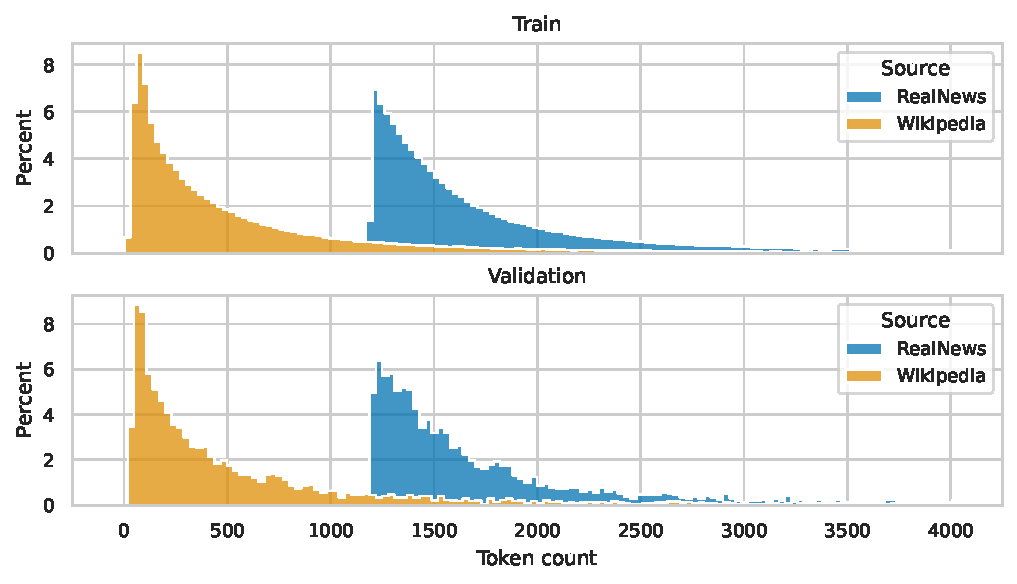
\includegraphics[width=\textwidth]{./img/val_data_dist.pdf}

  \caption{Distribution of train and validation documents' lengths for
  \Dataset{val-500k}.}

  \label{fig:val_data_dist}

\end{figure}

\section{Validation tasks}\label{section:validation_tasks}

We compare the embedding models based on their performance on
downstream tasks. We use a subset of our evaluation tasks, described in
detail in Chapter~\ref{chapter:evaluation}. We include tasks with either
a large enough training split suitable for cross-validation or a validation
split. All tasks are classifications evaluated using a validation
split, except for \Task{IMDB}, where we take the mean score of five
cross-validation folds. To make the validation faster to compute, we downsample
the validation and train splits to 10000 examples. We downsample the datasets
according to their label distribution so that the truncated split has a label distribution nearly identical to the original one. We present the validation
tasks and their document count in Table~\ref{table:validation_tasks}.

We use binary or micro-averaged accuracy as the scoring metric. Often, we need
to compare performance across several tasks. However, not all tasks are equally
difficult, so averaging accuracies would lead us to favor models that
performed well on easy tasks and undervalue models that performed well on
more difficult tasks. Therefore, we normalize the accuracy by the highest
score reached for the given task within the considered models,
making the tasks equally difficult. We call this metric \emph{normalized
accuracy}. When more tasks are taken into account, we asses models based on the
mean normalized accuracy. In visualizations, we mark mean normalized accuracy
with a black triangle.

When validating a trained embedding model on a task, we finetune a head that
transforms the embeddings into the output format required for the given task. We
do not finetune the embedding model itself. Besides speeding up the validation,
this gives us a more genuine picture of the embedding model's performance.
Since all our validation tasks are classifications, the heads are just 2-layer
neural network classifiers with a cross-entropy loss. We present the complete
list of the classifier's hyperparameters and training parameters in
Table~\ref{table:head_train_params}.

\begin{table}
  \footnotesize
  \centering
  \begin{tabular}{llrrrr}
    \toprule
      & \multicolumn{2}{c}{Documents} & Classes & \multicolumn{2}{c}{Class percentage} \\
    \cline{2-3} \cline{5-6}
      Dataset & Train & Validation & & Train & Validation \\
    \midrule
      \Task{arxiv} \citep{arxiv_papers} & \dag10 000 & 2 500 & 11 & 9.09$\pm$1.24\% & 9.09$\pm$1.01\% \\
      \Task{imdb} \citep{maas2011learning} & \dag10 000 & - & 2 & 50.00$\pm$0.00\% & - \\
      \Task{oc} \citep{zhou2020multilevel} & \dag10 000 & \dag10 000 & 2 & 50.00$\pm$0.06\% & 50.00$\pm$0.15\% \\
      \Task{aan} \citep{zhou2020multilevel} & \dag10 000 & \dag10 000 & 2 & 50.00$\pm$1.50\% & 50.00$\pm$4.57\% \\
      \Task{s2orc} \citep{zhou2020multilevel} & \dag10 000 & \dag10 000 & 2 & 50.00$\pm$0.09\% & 50.00$\pm$0.32\% \\
      \Task{pan} \citep{zhou2020multilevel} & \dag10 000 & 2 908 & 2 & 50.00$\pm$0.00\% & 50.00$\pm$0.00\% \\
    \bottomrule
  \end{tabular}

  \caption{Validation tasks we use to compare embedding models in this
  chapter. We truncated splits marked with {\dag} to speed up the evaluation
  process. We truncate a split by downsampling it according to its label
  distribution. The class distributions of all tasks are well balanced except
  for \Task{aan}, as can be seen from the mean and standard deviation of class
  percentages.}

  \label{table:validation_tasks}

\end{table}


\begin{table}
  \centering
  \footnotesize

  \begin{tabular}{l c}
    \toprule
    Parameter & Value \\
    \midrule
    Hidden features & 50 \\
    Hidden dropout rate & 0.5 \\
    Hidden activation & ReLU \\
    Epochs & 10 \\
    Batch size & 32 \\
    Weight decay & 0.1 \\
    Label smoothing & 0.1 \\
    Learning rate & 1e-4 \\
    Learning rate decay & Cosine \\
    Maximum gradient norm & 1.0 \\
    Optimizer & AdamW \\
    Mixed-precision training & Yes \\
    \bottomrule
  \end{tabular}

  \caption{Hyperparameters used for training classification heads during
  evaluation in this chapter.}

  \label{table:head_train_params}

\end{table}

\section{Student's model configuration and baselines}\label{section:student_model_config_baselines}

As we explained in Section~\ref{section:student_model}, we initialize our
student model with Longformer \citep{beltagy2020longformer}. We use
Longformer's base version with about 126M parameters implemented by HuggingFace
\texttt{transformers}
library\footnote{\url{https://huggingface.co/allenai/longformer-base-4096}}.

We pool the last layer's hidden states and compute their mean to obtain the
input's embedding. We do not use global attention and employ sliding window
attention, with the window sizes $\omega$ set to the default 512 tokens. In our
preliminary experiments, we also tested using global attention to the
\texttt{CLS} token and taking its hidden state from the last layer as the
input's embedding. However, the mean-pooling approach proved to be superior.
Additionally, with mean-pooling, we found global attention is not beneficial,
so we avoided it.

We aim for fast convergence with a small
memory footprint when we train the student model. We, therefore, use a high learning rate, no gradient accumulation
steps, mixed-precision training, and gradient checkpointing. We enumerate the
complete list of student's training parameters in
Table~\ref{table:student_train_params}. We use these values for all student's
training in this chapter.


\begin{table}
  \centering
  \footnotesize

  \begin{tabular}{l c}
    \toprule
    Parameter & Value \\
    \midrule
    Batch size & 6 \\
    Weight decay & 0.1 \\
    Learning rate & 1e-4 \\
    Learning rate decay & Cosine \\
    Maximum gradient norm & 1.0 \\
    Optimizer & AdamW \\
    Gradient accumulation steps & 1 \\
    Warmup steps & 10\% of training steps \\
    Gradient checkpointing & Yes \\
    Mixed-precision training & Yes \\
    \bottomrule
  \end{tabular}

  \caption{Training parameters' values we use every time we train a student model in this chapter.}

  \label{table:student_train_params}

\end{table}

\subsection{Baselines}

As mentioned, we aim to finetune our training
method so the student model surpasses teachers and Longformer. To check
how close we are to this goal throughout this chapter, we compare the student
variants to three models: Longformer \citep{beltagy2020longformer}, SBERT
\citep{reimers2019sentence}, and PV \citep{le2014distributed}. We compare
students to Longformer to judge how our training method improves document
embeddings. As we mentioned above, we use a subset of Longformer's pre-training
data. So, the student model can't gain performance just due to
the training data since it has seen the same data during
pre-training. For context, we train the student models for only 3.8\%
iterations of Longformer's pre-training with an eight times smaller batch size.

We compare the students to the two teachers to see how much performance our
training method ignores or takes advantage of. If our student model performs
worse than a particular teacher, we need to improve how we distill the
teacher's embeddings into the student's embeddings. As the student has
architectural advantages compared to both teachers, such as longer maximum
context, we hypothesize it can match and surpass both teachers' performance. We
discuss the configuration of the structural teacher in the following section.
Paragraph Vector's training is a part of our training method, so we discuss
further details in Section~\ref{section:pv_training}, where we experiment with
PV's training hyperparameters.

\section{Structural loss}\label{section:structural_loss}

We start our experiments with the structural loss $\Loss_S$. The structural
loss compares the student's and the structural teacher's embeddings. Its
goal is to encourage distillation of the quality of the structural teacher's
embeddings into the student's embeddings. We focus on the structural loss first
since, in our preliminary experiments, we observed that the structural quality
is more significant to the performance of the student model than the contextual
quality. We arrive at the same conclusions later in this chapter in
Section~\ref{section:projections_only_contextual}. Therefore, we prioritize
first finding the best-performing hyperparameters of the structural loss and
adapting the contextual loss to it afterward.

As we mention in Section~\ref{section:teacher_models}, we use SBERT
\citep{reimers2019sentence} as our structural teacher. We use SBERT's version
initialized with MPNet \citep{song2020mpnet} since it is a relatively small
model with above-average
performance\footnote{\url{https://sbert.net/docs/pretrained_models.html}}. We
use SBERT's implementation from the HuggingFace \texttt{transformers}
library\footnote{\url{https://huggingface.co/sentence-transformers/all-mpnet-base-v2}}
with a mean pooling layer above the last layer's hidden states. We do not
perform any finetuning and use the pre-trained weights only.

As explained in Section~\ref{section:abstract_loss}, we choose structural loss
to be more restrictive, forcing an exact similarity between the two embeddings.
Therefore, we test two different exact losses as structural losses: Mean Squared
Error (\emph{MSE}) and cosine distance. We try MSE because it forces
equality, the most restrictive similarity measure. The motivation for using
cosine comes from the embeddings' use cases, where cosine distance is a popular
similarity measure. More importantly, it is also used by SBERT's authors,
suggesting that for SBERT's embeddings, it is the best-performing similarity
measure.

We train the student model with each loss on the first 15k documents of
\Dataset{val-500k} with the hyperparameters given in
Section~\ref{section:student_model_config_baselines}. As we show in
Figure~\ref{fig:structural_basic}, with cosine distance, the student model
surpasses both baselines. The fact that the student performs better
than the teacher indicates that Longformer's longer context and supervision from
the structural teacher can boost the student's performance even above the level
of the teacher. Moreover, SBERT's scores are significantly higher than
Longformer's, showing that unless Longformer's embeddings are finetuned, its
longer context length or pre-training is of no benefit.

These encouraging results show that using just the structural teacher can be a
valid method of improving a model's embeddings. However, we hope to
enhance the student's performance even further. In subsequent experiments, we
use cosine as the structural loss. For brevity, we label the student model
trained with just the structural loss as \Model{only-structural;cosine}.

\begin{figure}
  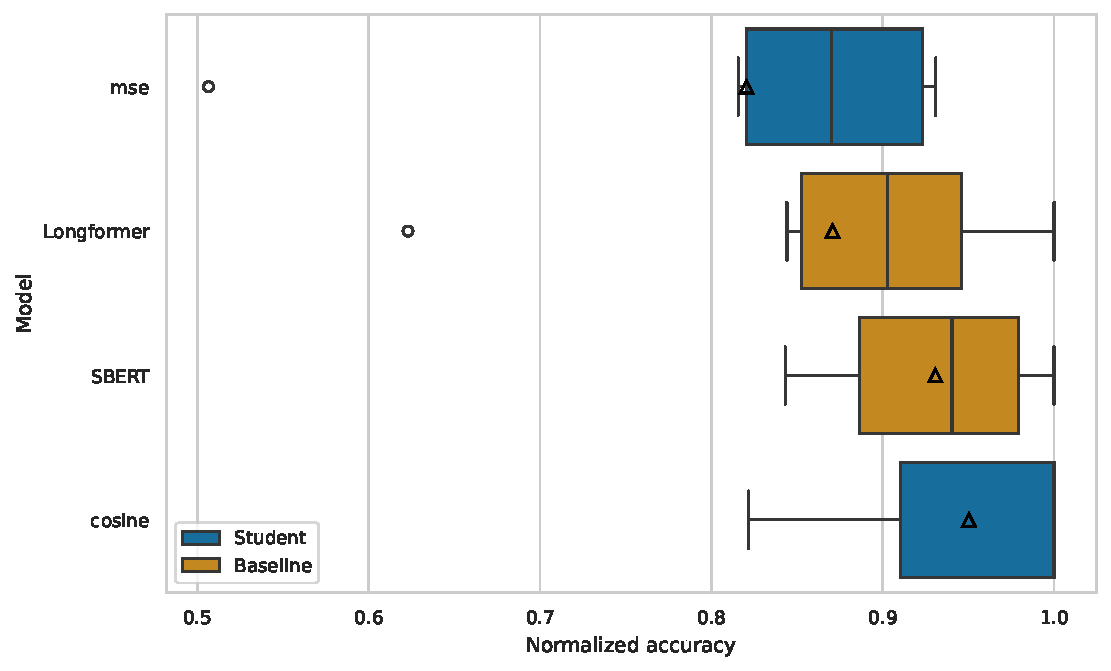
\includegraphics[width=\textwidth]{img/structural_simple_losses.pdf}

  \caption{Performance of student models trained with just the structural
  teacher.}

  \label{fig:structural_basic}
\end{figure}

\subsection{Composite structural losses}\label{section:composite_losses}

Besides the cosine and the MSE, we also explore losses that combine a positive
and a negative component, such as max-marginals or contrastive loss. We call
such losses \emph{composite} as opposed to the \emph{simple} losses, such as
MSE or cosine distance. In composite losses, the positive component compares
the student's and the corresponding teacher's embedding and rewards the model
if they are similar. The negative component compares the student's embedding of
an input and the teacher's embedding of a different input and punishes the
model if they are similar. For brevity, we call the teacher's embedding corresponding to the same input positive, while the ones corresponding to
a different input negative.

Our initial motivation behind the composite losses was that the negatives could
give the model a more precise indication of where it should move its embeddings in
the vector space. Therefore, it could converge faster to the structural
teacher's embeddings. However, as we discuss in
Section~\ref{section:composite_analysis}, this is not what happens.
Nevertheless, some of the models performed so well that we do not want to overlook
these losses as they might be beneficial for future research.

We explored two types of composite losses: max-marginals and contrastive. To
formulate these losses, we label the student's embedding as $y$, the
corresponding teacher's embedding as $y_{\text{pos}}$, the set of negatives as
$Y_{\text{neg}}$, the given similarity measure as $\operatorname{sim}$, and a
weighting parameter as $\gamma$. We define the max-marginals loss in
Equation~\ref{eq:max_marginals} and the contrastive loss in
Equation~\ref{eq:contrastive}.


\begin{equation}
  \Loss_{\text{max-marginals}}(y, y_\text{pos}, Y_\text{neg}) =
    \operatorname{sim}(y, y_\text{pos}) -
    \gamma \frac{1}{|Y_\text{neg}|} \sum_{y_\text{neg} \in Y_\text{neg}}
      \operatorname{sim}(y, y_\text{neg})
  \label{eq:max_marginals}
\end{equation}

\begin{equation}
  \Loss_{\text{contrastive}}(y, y_\text{pos}, Y_\text{neg}) =
    -\log \frac{
      \exp(\cos(y, y_\text{pos}))
    }{
      \exp(
        \cos(y, y_\text{pos}) +
        \sum_{y_\text{neg} \in Y_\text{neg}} \cos(y, y_\text{neg})
      )
    }
  \label{eq:contrastive}
\end{equation}

For max-marginals loss, we try MSE and cosine distance as
$\operatorname{sim}$ and simultaneously try several weightings $\gamma$. We
compare models trained with the composite losses with those trained with the
simple losses in Figure~\ref{fig:structural_composite_vs_simple}. Composite
losses using MSE seem to benefit from the negative loss component, as 3 out of 4 outperform the simple MSE loss. However, the benefit is significant enough to surpass the two baselines for only one version. With cosine, it seems that
  the negative loss component hurts the performance since only one version
  outperforms the simple cosine loss and does so by only $10^{-4}$. In the subsequent section, we carry out an analysis to explain the differences between the behaviors of MSE and cosine composite losses.

\begin{figure}

  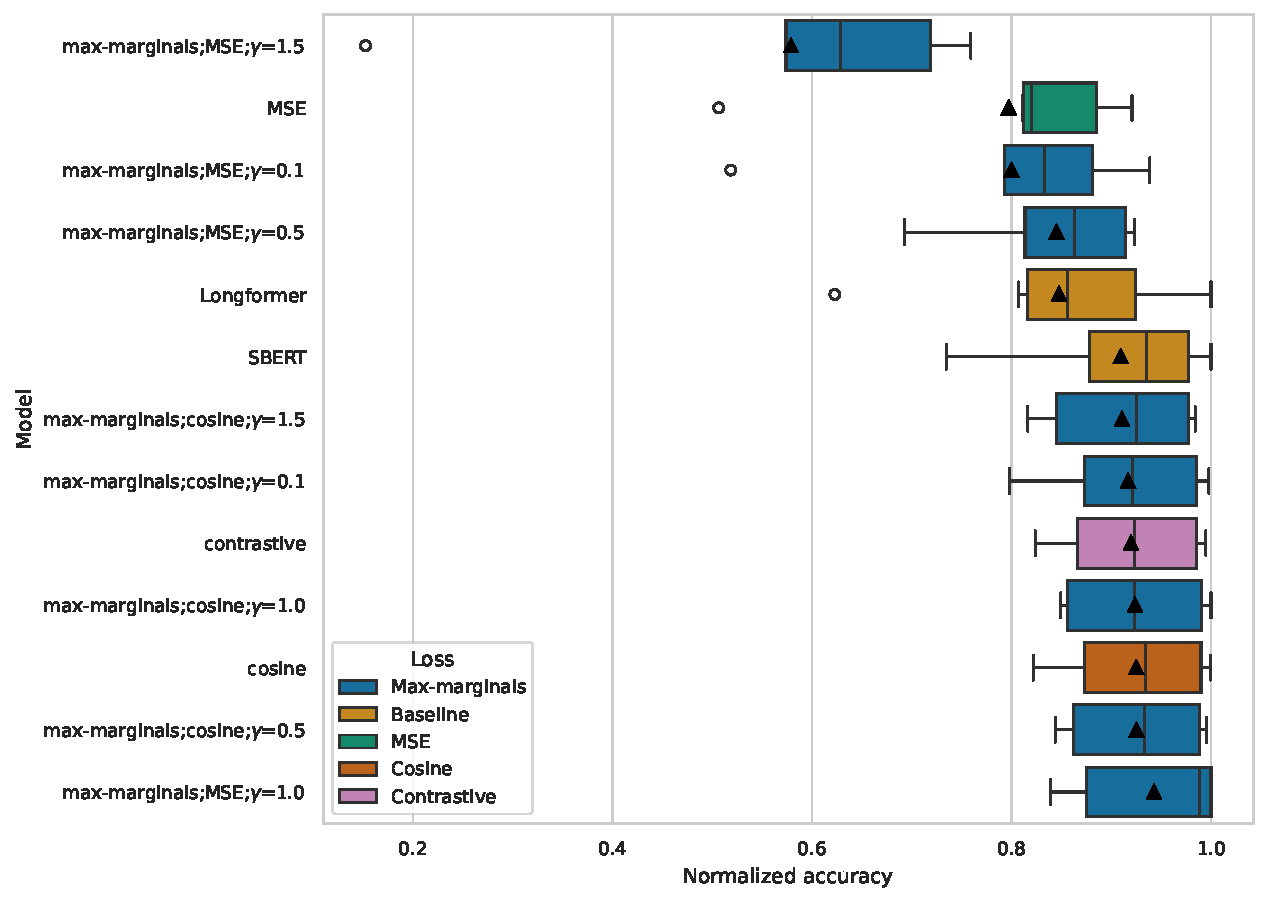
\includegraphics[width=\textwidth]{./img/structural_both_losses.pdf}

  \caption{Performance of student models trained with composite and simple
  structural losses.}

  \label{fig:structural_composite_vs_simple}
\end{figure}

\subsubsection{Analysis of composite losses}\label{section:composite_analysis}

The results of composite losses presented in
Figure~\ref{fig:structural_composite_vs_simple} suggest that the composite
losses using MSE benefit from the negative loss component, whereas the ones
using cosine do not. Furthermore, for most MSE max-marginals losses, the
benefit of the negative loss component is only minimal. To explain these
results, we compare the distances to positives and negatives for several chosen
models in Figure~\ref{fig:composite_distances}. Composite losses using MSE
widen the gap between positives and negatives at the expense of increasing the
distance to positives. So, the benefit of the negative component is not that it
gives a more precise training signal and causes a faster convergence to the
structural teacher's embeddings. Conversely, the benefit comes from a more
apparent separation between embeddings of different documents, even if the
generated embeddings do not correspond to the teacher's embeddings well. The
situation is different for cosine since its range is limited. Therefore, the
only option to increase the gap between the positives and the negatives is to
decrease the distances to the positives. Besides, all of the negatives are
almost perpendicular to the generated embedding and, therefore, direct the
generated embedding in only one dimension out of the 768. Consequently, the
benefit of the negative component in cosine composite losses is minimal.

\begin{figure}
  \centering
  \begin{subfigure}{\textwidth}
    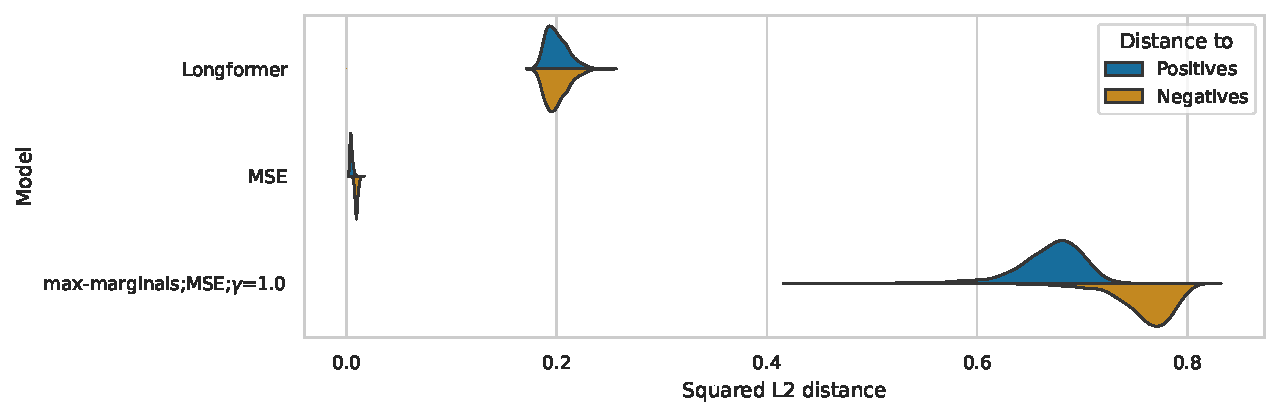
\includegraphics[width=\textwidth]{img/composite_mse_distances.pdf}
    \caption{With MSE}

    \label{fig:composite_mse_distances}

  \end{subfigure}
  \begin{subfigure}{\textwidth}

    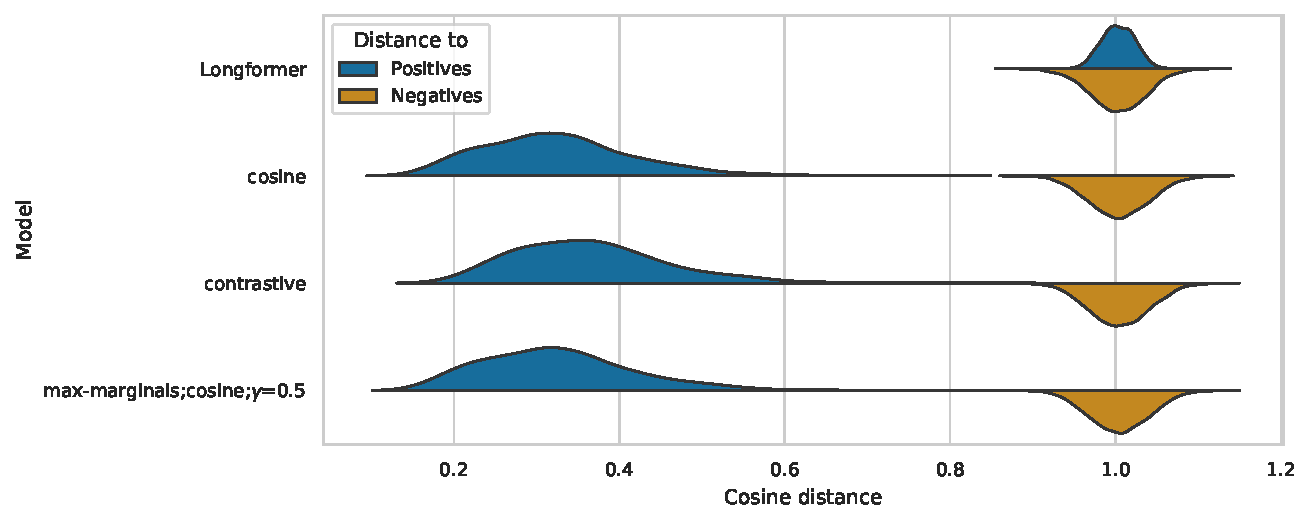
\includegraphics[width=\textwidth]{img/composite_cos_distances.pdf}
    \caption{With cosine}

    \label{fig:composite_cos_distances}
  \end{subfigure}

  \caption{Distribution to distances between the model's and the structural
  teacher's embeddings. A distance to the teacher's embedding of the same
  document is labeled as \emph{positive}, whereas distances to the teacher's
  embedding of another document are labeled as \emph{negative}. We generated
  the distances from the first 1000 documents of \Dataset{val-500k}'s
  validation split.}

  \label{fig:composite_distances}

\end{figure}

Contrary to our initial hypothesis, the negative loss component does not ensure
faster convergence of the student's embeddings to those of the structural
teacher. The negative component causes the student's embedding to move away
from the structural teacher's embedding and, hence, goes against the goal of
our training. Nonetheless, as we do not want to throw away a well-performing
model and are interested in how the composite loss cooperates with a contextual
loss, we keep experimenting with the best-performing composite loss in the
following sections. Nonetheless, the pure cosine loss remains the preferred
structural loss since it is consistent with the goal of our training. For
brevity, we label the student model trained with just the max-marginals MSE
structural loss, with $\gamma=1.0$ as \Model{only-structural;mm-MSE}.

\section{Structural and contextual loss}\label{section:structural_and_contextual}

This section explores contextual losses that complement the best-performing
structural and composite structural loss we selected in the previous section.
Since there are several hyperparameters to explore, we split this section into
parts. Each part focuses on a different aspect of the contextual loss or the
weighting of the contextual and structural loss. At the end of each part, we
select a few best-performing variants, which serve as a starting point for the
subsequent section. First, we must train the contextual teacher to experiment
with the contextual loss. We do so in Section~\ref{section:pv_training}, where
we train several Paragraph Vectors and pick the most promising ones. Then, we
experiment with the contextual loss's configuration for all selected Paragraph
Vectors in Section~\ref{section:contextual_loss}. To illustrate the importance
of the structural teacher, we show the performance we reach when we use only
the contextual loss. More importantly, we test the contextual losses with
cosine and max-marginals MSE structural losses. We pick the best-performing
combination of the contextual loss and the contextual teacher for each
structural loss. Finally, we explore different ways to weigh the contextual and
structural loss for each of the two combinations in
Section~\ref{section:weighting_experiments}.

\subsection{Optimizing Paragraph Vector's training}\label{section:pv_training}

We choose Paragraph Vector \citep{le2014distributed} as our contextual teacher,
as we elaborate on in Section~\ref{section:paragraph_vector}. Since there is no
concept of a pre-trained PV, as in the case of transformers, we train PV from
scratch. We use PV's implementation from the Gensim
library\footnote{\label{fn:link_to_gensim}\url{https://radimrehurek.com/gensim}}
and explore some of the hyperparameters that govern the training of PV. We
focus on four hyperparameters that we consider important and adopt the
recommendation of the library or related literature. We enumerate the adopted
and the grid-searched hyperparameters in Table~\ref{table:pv_hyperparams}. To
explain the meaning of all hyperparameters, we provide the following summary:


\begin{itemize}

  \item \texttt{dm} --  PV architecture; true for Distributed Memory (DM),
    false for Distributed Bag of Words (DBOW)

  \item \texttt{vector\_size} -- dimensionality of the generated embedding

  \item \texttt{min\_count} -- words with document frequency below this limit
    will be ignored

  \item \texttt{text\_pre\_process} -- applied word processing done before the
    model's training; for stemming, we use PorterStemmer implemented by the \texttt{nltk}
    library\footnote{\url{https://www.nltk.org/api/nltk.stem.porter.html}}

  \item \texttt{negative} -- number of noise words used for negative sampling
    during training

  \item \texttt{window} -- the maximum distance between known and predicated
    word

  \item \texttt{sample} -- percentile threshold configuring which words will be
    downsampled; 0 for no downsampling


  \item \texttt{dbow\_words} -- whether to train word embeddings using
    Word2Vec's \citep{mikolov2013efficient} Skip-gram architecture together
    with document embeddings; only applicable to DBOW, as DM learns word embeddings by default

  \item \texttt{epochs} -- a number of iterations done over the corpus during
    training

\end{itemize}


As recommended by the authors of PV \citep{le2014distributed}, we experiment
with both architectures. For each architecture, we try different values of
\texttt{vector\_size}, \texttt{min\_count}, and \texttt{text\_pre\_process},
which all control the model's regularization. Settings such as higher
dimensional embedding, small minimum count, and no text pre-processing
regularize the model the least. They give the model the most information on its
inputs while providing it with large embedding through which it
can express precisely. On the other hand, using lower dimensional embedding,
large minimum count, and stemming the document's words forces the model to be
more general and less precise. The model has less detailed information on its
input and must squeeze all of it into a small vector. We do not see any value in
trying dimensions of embeddings higher than 1024 since, in later experiments, we
must distill the contextual embedding to a 768-dimensional embedding of our
student model. Intuitively, the larger the contextual embedding will be,
the smaller the fraction of information the student model will be able
to digest. Also, there is no value in considering \texttt{min\_count} to be
lower than two since we would only add words unique to a single
document. Embeddings of such words would be poorly trained and not add
meaningful information to the document's embedding. The last hyperparameter that is
worth mentioning is \texttt{dbow\_words}. DBOW, on its own, does not train word
embeddings, which are, by default, randomly generated. Setting \texttt{dbow\_words} to true
causes DBOW also to train word embeddings using Word2Vec's Skip-gram model
\citep{mikolov2013efficient} in each epoch. \cite{lau2016empirical} showed that
random word embeddings significantly hurt the model. Consequently, when
training DBOW, we also train word embeddings despite the slower training, which
it inevitably causes.

\begin{table}
  \footnotesize
  \centering
  \begin{tabular}{lrc}
    \toprule
    Hyperparameter & Value(s) & Recommended by \\
    \midrule
    \texttt{dm} & true, false & - \\
    \texttt{vector\_size} & 100, 768, 1024 & - \\
    \texttt{min\_count} & 2, 10\% of training corpus& - \\
    \texttt{text\_pre\_process} & stem, lowercase, none & - \\
    \texttt{window} & 5 & default \\
    \texttt{negative} & 5 & default, \cite{lau2016empirical} \\
    \texttt{sample} & 0 & default \\
    \texttt{dbow\_words} & true & \cite{lau2016empirical} \\
    \texttt{epochs} & 10 & default, \cite{dai2015document} \\
    \bottomrule
  \end{tabular}

  \caption{Used hyperparameters for training Paragraph Vector. We grid-searched
  four hyperparameters: PV architecture, vector size, minimum word count, and
  pre-processing of words. For the rest of the hyperparameters, we adopted either the
  default values or recommended by the mentioned literature.}

  \label{table:pv_hyperparams}

\end{table}

We train all variants on the whole \Dataset{val-500k} corpus. We follow the
recommendations of \cite{le2014distributed} and also evaluate the combination of
both architectures. However, we only select the best three models
from each architecture and evaluate all nine combinations. We call these models
\emph{compound} Paragraph Vectors. In total, there are 45 models whose
performance on validation tasks we report in Figure~\ref{fig:pv_val_scores}.
The single models favor large embedding dimensions and low minimum count. Additionally, on average, stemming or lowercasing leads to higher scores
than not pre-processing the words. DBOWs vary more in performance,
occupying the best and the worst positions, whereas DMs are more
consistent. We achieve a slight improvement by concatenating a DM and a DBOW
model, but considering the resulting model has an embedding twice as large, the improvement is not surprising. Interestingly, all compound models
perform very similarly, suggesting that slight imperfections of one model can
be compensated by another model of a different architecture.

\begin{figure}

    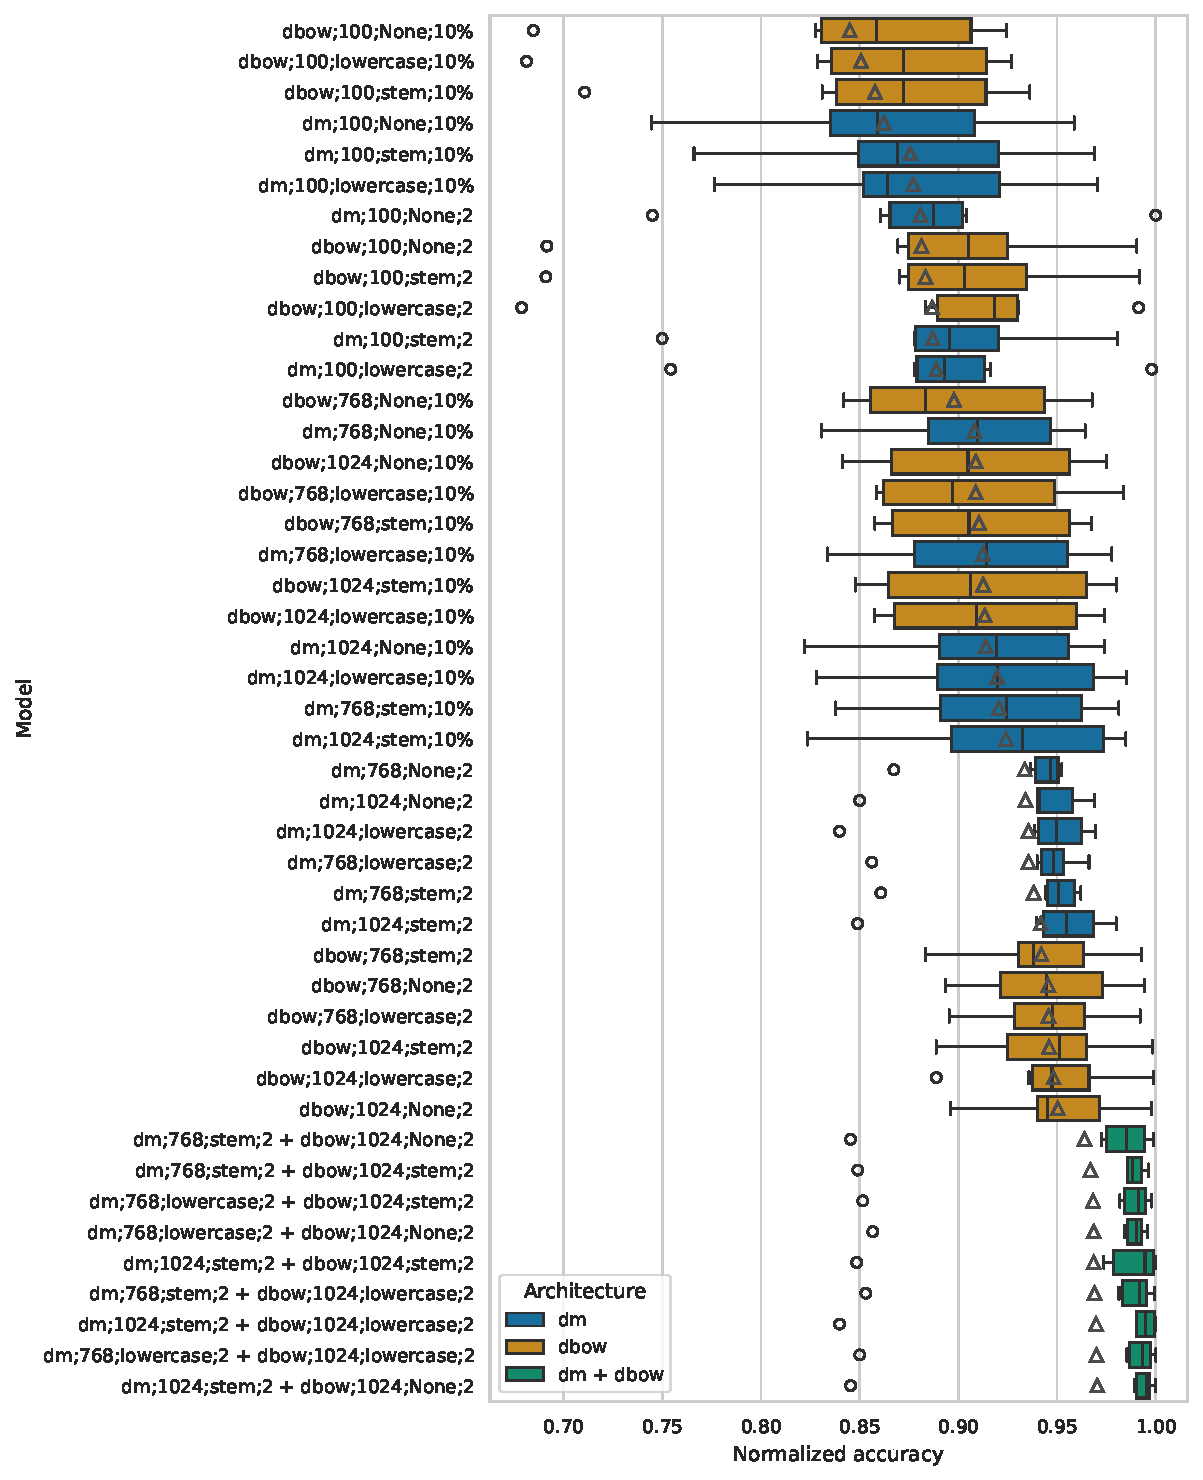
\includegraphics[width=\textwidth]{./img/pv_val_scores.pdf}

    \caption{Performance of all Paragraph Vector variants on validation tasks.
    We identify a model by its architecture, embedding dimension, text
    pre-processing, and minimum count. Compound models are identified as a concatenation of such identifiers separated
    by $+$.}

    \label{fig:pv_val_scores}

\end{figure}

In our preliminary experiments, we saw that the dimension of contextual
teacher embedding plays a significant role in teacher-student training.
So, we select three paragraph vectors with varying vector sizes. We pick the
best model with small vector size (\Model{DM;100;lowercase;2}), the best
single model (\Model{DBOW;1024;None;2}) and the best model composed of both
architectures (\Model{DM;1024;stem;2+DBOW;1024;None;2}). For brevity we label
these models as \Model{DM;100d}, \Model{DBOW;1024d} and \Model{PV;2048d} respectively.

\subsection{Contextual loss}\label{section:contextual_loss}

Contextual loss $\Loss_C$ compares the student's and the contextual teacher's
embeddings and encourages distillation of the quality of the teacher's
embedding into the student's embedding. As we discuss in
Section~\ref{section:abstract_loss}, we choose $\Loss_C$ to be less strict and
give the student model more freedom in encoding information into the
document embedding. Consequently, we do not consider losses such as MSE or
cosine since they enforce either an exact vector or a direction in the
embedding space. Instead, we use a variant of \emph{Canonical Correlation
Analysis} \citep{hotelling1992relations} (\emph{CCA}). In its base form, CCA
computes a correlation of two linearly projected sets of vectors, where the
projections are optimized to maximize the correlation. We define CCA
in Equation~\ref{def:cca_more_dim}.

\begin{defn}[Canonical Correlation Analysis]\label{def:cca_more_dim}

  For two matrices $X_1 \in \mathbb{R}^{n_1 \times m_1}$ and $X_2 \in
  \mathbb{R}^{n_2 \times m_1}$, Canonical Correlation Analysis for $k$
  dimensions finds $P \in \mathbb{R}^{m_1 \times k}$ and $Q \in \mathbb{R}^{m_2
  \times k}$ that maximize

  \begin{equation}
    \begin{split}
      &\CCA(X_1, X_2) = \sum_{i = 1}^k \corr(X_1P_{*i}, X_2Q_{*i}) \\
      \text{s.t.}\quad &P^TX_1^TX_1P = I_k = Q^TX_2^TX_2Q \\
    \end{split}
  \end{equation}


\end{defn}

CCA gives the student the freedom to change its embeddings as long as their
linear projections correlate more with the linear projections of the contextual
teacher's embeddings. However, linear projection may still leave too little
leeway for the student model to simultaneously mimic the structural teacher
while increasing the correlation with the projected contextual teacher's
embeddings. Ideally, we would like to adjust the strength of the projections and
thus regulate how exact the correlation between the student's and the
teacher's embeddings should be. Such adjustment is possible with \emph{Deep CCA}
(\emph{DCCA}) \citep{andrew2013deep}. DCCA projects the input vectors with two
neural networks and feeds the projections to the vanilla CCA. The two
networks are trained jointly with the embedding model based on
the computed CCA, which is used as a loss. The advantage of DCCA is that we can
adjust the strength of the projections and thereby regulate the pressure the
contextual loss inflicts on the student model. The larger the neural network
is, the more it can transform the embeddings and the less the student model needs to adjust its embedding.

As we can see in Equation~\ref{def:cca_more_dim}, CCA is computed from the
entire dataset of input vectors. And so DCCA is trained using a full-batch
optimization \citep{andrew2013deep} or a mini-batch optimization with large
batch sizes \citep{wang2015unsupervised}. However, both methods need large
amounts of GPU memory and are suitable only with smaller models. For
this reason, we avoid CCA and use SoftCCA \citep{chang2018scalable} instead.
SoftCCA reformulates CCA such that it is usable even in the case of mini-batch
optimization with small batches. To explain how SoftCCA is related to CCA, we
reformulate the solution to CCA using a Forbenious matrix norm in
Equations~\ref{def:cca_with_forbenious_first}-\ref{def:cca_with_forbenious_last}.

\begin{align}
  P^\ast, Q^\ast &= \underset{P, Q}{\argmin} ||X_1P - X_2Q||^2_F \label{def:cca_with_forbenious_first} \\
  &= \underset{P, Q}{\argmin} \trace\left((X_1P - X_2Q)^T(X_1P - X_2Q)\right) \\
  &= \underset{P, Q}{\argmin} {-2} \trace(P^TX_1^TX_2Q) \\
  &= \underset{P, Q}{\argmax} \trace(P^TX_1^TX_2Q) \\
  &= \underset{P, Q}{\argmax} \sum_{i = 1}^k \corr(X_1P_{*i}, X_2Q_{*i}) \label{def:cca_with_forbenious_last}
\end{align}

Thus, by minimizing CCA, we effectively minimize the difference between two
projections with uncorrelated features. SoftCCA enforces the same behavior with
two separate losses:

\begin{itemize}

  \item L2 loss, which minimizes the difference between projections:

    \begin{equation}
      \Loss_{\text{L2}}(X_1, X_2) = ||X_1 - X_2||^2_F = \MSE(X_1, X_2)
    \end{equation}

  \item \emph{Soft Decorrelation Loss} (\emph{SDL}), which forces a projection
    to have decorrelated features:

    \begin{equation}
      \Loss_{\text{SDL}}(X^t) = \sum_{i \ne j} \left|
          \frac{(\Phi^t_X)_{ij}}{\hat{\beta}^t}
          \right|
    \end{equation}
    where
    \begin{align}
      \Phi^t_X &= \beta \Phi^{t-1}_X + \Sigma_{X^t} \\
      \Phi^0_X &= \bm{0}_d \\
      \hat{\beta}^t &= \beta \hat{\beta}^{t-1} + 1 \\
      \hat{\beta}^0 &= 0
    \end{align}

\end{itemize}

Where

\begin{itemize}

  \item $X, X_1, X_2 \in \mathbb{R}^{b \times d}$ are mini-batches of
    $d$-dimensional vectors

  \item $\Sigma_{X}$ is a covariance matrix of a mini-batch of vectors $X$

  \item $\bm{0}_d$ is a $d \times d$ zero matrix

  \item $\beta$ is a hyperparameter

  \item $\Phi_X^t, X^t, \hat{\beta}^t$ is $\Phi_X, X, \hat{\beta}$ at iteration
    $t$

\end{itemize}

The L2 loss forces the projected vectors to be equal, while the Soft
Decorrelation Loss forces them to have uncorrelated features. Notice that to
have a better estimate of the projected vector's covariance matrix, SDL keeps a
running mean. Similarly to Batch Normalization \citep{ioffe2015batch}, SDL
updates the running mean during training but avoids any updates during
inference. With the above losses and the weighting hyperparameter
$\delta$, we define SoftCCA in Equation~\ref{eq:soft_cca}.

\begin{equation}\label{eq:soft_cca}
  \Loss_{\text{SoftCCA}}(X_1, X_2) = \Loss_{\text{L2}}(X_1, X_2) +
      \delta ( \Loss_{\text{SDL}}(X_1) + \Loss_{\text{SDL}}(X_2) )
\end{equation}

We use SoftCCA loss as a replacement for CCA in DCCA. To be explicit, we
project the student's and the contextual teacher's embedding with two separate
feed-forward neural networks. Then, we apply SoftCCA loss, which provides
a training signal for the embedding model and the neural
networks projecting the embeddings. For brevity, we call the neural networks
projecting an embedding \emph{student} and \emph{contextual projections}, depending on which embedding they project. And so, we can finally express $\Loss_C$ from Equation~\ref{eq:abstract_loss} more concretely.
For a student projection $f_\Student$ and a contextual projection $f_C$, we
formulate our contextual loss in Equation~\ref{eq:contextual_loss}. We also
illustrate the architecture of contextual loss graphically in
Figure~\ref{fig:contextual_loss}.

\begin{equation}\label{eq:contextual_loss}
  \Loss_C(y_\Student, y_{\Teacher_C}) = \Loss_{\text{SoftCCA}}(
    f_\Student(y_\Student),
    f_C(y_{\Teacher_C})
  )
\end{equation}

\begin{figure}

  \centering
  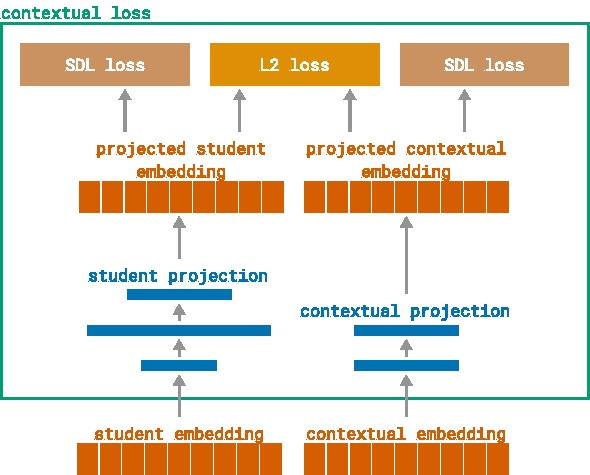
\includegraphics[width=0.7\textwidth]{img/contextual_loss.pdf}

  \caption{Architecture of contextual loss.}

  \label{fig:contextual_loss}

\end{figure}

In our preliminary experiments, we found that the value of $\delta$ from
Equation~\ref{eq:soft_cca} has little effect on the final student's
performance. So, we set it so that the ranges of $\Loss_{\text{L2}}$ and
$\Loss_{\text{SDL}}$ are roughly equal and leave it as so. On the other hand,
choosing the right value of $\beta$ proved to be critical. Based on how the CCA
of the projected embeddings of the validation split progressed throughout the
training, we found the optimal value to be 0.95, which puts a relatively large
emphasis on the accumulated mean compared to lower values of $\beta$.

In the rest of this section, we experiment with the strength of the
projections. In the following section, we build the basic intuition behind
training with the two projections and SoftCCA while finding the ideal
contextual projection without structural loss. In the subsequent sections,
we study how different structural losses influence the projections. First, we
experiment with cosine and then with max-marginals MSE loss. In all cases, we
test the projections for each of the three contextual teachers:
\Model{DM;100d}, \Model{DBOW;1024d} and \Model{PV;2048d}. Finally, we select
the best contextual loss with the best contextual teacher for both cosine and
max-marginals MSE structural loss, with which we experiment in
the subsequent section.

\subsubsection{Contextual projection with contextual loss
only}\label{section:projections_only_contextual}

With only the contextual loss, the student's only goal is to mimic the
contextual teacher. This presents an elementary setting in which we can study
the behavior of the projections and the contextual loss as a whole without
any influence from the structural loss.

Our preliminary experiments show that the projections' over-parameterization hurts the model's performance. Even though large projections
result in smaller SoftCCA loss, they tend to harm the CCA computed on the student's and
contextual teacher's embeddings. Strong projections compensate for the
student's flaws, lessening the pressure on the student model as it does not
need to adjust its embedding much. Consequently, the student model
learns very little compared to the projections. Similarly, strong contextual
projection takes away pressure from the student projection and vice-versa. In
this regard, it is essential to keep the contextual projection small. This puts more pressure on the student's side, where the gradients can
propagate to the embedding model.

As we mentioned before, we feed the projected outputs to SoftCCA loss
$\Loss_{\text{SoftCCA}}$. As SoftCCA requires both inputs to be of the same
dimension, both projections must end with an equally sized layer. We always use
the dimension of the larger embedding as the final projection dimension. We do
so to preserve all the embeddings' information through the projection and
force the student model to distill all contextual embedding's dimensions, not just their subset. Also, there is no point in projecting the
embeddings to even more dimensions than the embeddings have. Due to
the Pigeonhole principle, some features of the final projections would have to
depend on the same embedding's features and, therefore, would correlate with each
other. Such correlations would create unnecessary conflict with the SDL loss. This phenomenon would also
occur for projections with an hourglass shape, where there is one
bottle-neck layer with significantly fewer dimensions than the layers after or
before it. And indeed, during preliminary testing, we saw these projections
always perform poorly.

We build the projections as a sequence of blocks, where each block is composed
of a fully connected layer and an optional Rectified Linear Unit (\emph{ReLU}).
In preliminary experiments, we also tried adding Dropout, Batch, or Layer Normalization layers at different places in a block. However, in all cases, they had either
negligible or negative effects on the performance of the final model. We label
each block with the dimension of the fully connected layer and with the
activation's name in brackets if used. We identify a projection by block's labels delimited by an ``x''. So, \Proj{768(ReLU)x1024} are two feed-forward layers with 768 and 1024 features connected via ReLU. To
label projections without any layers, we use a dash. We present all the
projections' variations we tested in Table~\ref{table:contextual_projections}.
Considering the conditions described in the previous paragraph, we choose a
strong and a weak projection for both the student and contextual side. We are
careful not to over-parametrize either projection and lean toward stronger
student projection.

\begin{table}
  \centering
  \footnotesize

  \begin{tabular}{lrrr}
    \toprule
      & \multicolumn{3}{c}{Contextual teacher's embedding dimension} \\
      \cline{2-4} \\
      Projection & 100 & 1024 & 2048 \\
    \midrule
      \multirow[t]{2}*{Student} & \Proj{768(ReLU)x1024(ReLU)x768} & \Proj{768(ReLU)x1024} & \Proj{1024(ReLU)x2048} \\
      & \Proj{768} & \Proj{1024} & \Proj{2048} \\
      \multirow[t]{3}*{Contextual} & \Proj{100(ReLU)x768} & \Proj{768x1024} & \Proj{1024x2048} \\
      & \Proj{768} & \Proj{1024} & \Proj{2048} \\
      & & - & - \\
    \bottomrule
  \end{tabular}

  \caption{All tested variants of projections with only contextual loss. We do
  a grid search of the given variants for each contextual teacher. This results
  in 16 combinations overall.}

  \label{table:contextual_projections}
\end{table}

We train the student models on the first 15k documents of \Dataset{val-500k}
and compare the models' performance to all the relevant teachers, Longformer
and \Model{only-structural;cosine} in Figure~\ref{fig:projections_contextual}.
We identify a student model with the contextual teacher's dimension, the
student projection prefixed by \Model{S:} and the contextual projection
prefixed by \Model{C:}.

The results correspond to those we witnessed in our preliminary experiments and
showcase some of the mentioned projections' behaviors. The better half of the
student models differs from the rest by having a minimal contextual projection.
Moreover, for a given contextual teacher and a projection, the student model
with a larger student projection outperforms the student with a smaller one in
all cases but one.

Half of the tested projections improve the score of Longformer. The better projections demonstrate
that we can distill useful information from the contextual teacher to
the student, while the worse projections highlight how important the projections are. However,
as our contextual loss does not enforce an exact similarity of the student's and
the contextual teacher's embedding, most students do not outperform
their respective contextual teachers. Interestingly, students trained with
\Model{DM;100d} surpass students trained with better performing
\Model{DBOW;1024d}. We can observe the same performance differences for
\Model{DBOW;1024d} and \Model{PV;2048d}, even if we compare projections that
scale with the contextual embedding, such as \Proj{1024d;S:1024;C:-} and
\Proj{2048d;S:2048;C:-} or \Proj{1024d;S:1024;C:1024} and
\Proj{2048d;S:2048;C:2048}. Consequently, distilling
information from an embedding with fewer features seems easier than from a larger one. And
so, even though PV with 2048 dimensions beats SBERT, the students trained with
it fail to capitalize on this advantage and perform worse than the model
trained with SBERT. Therefore, we conclude that according to our results, the
structural teacher is more important to the student's performance than the
contextual teacher and justifies why we search for the ideal contextual loss to
the best performing structural loss rather than the other way around.

\begin{figure}

  \centering

  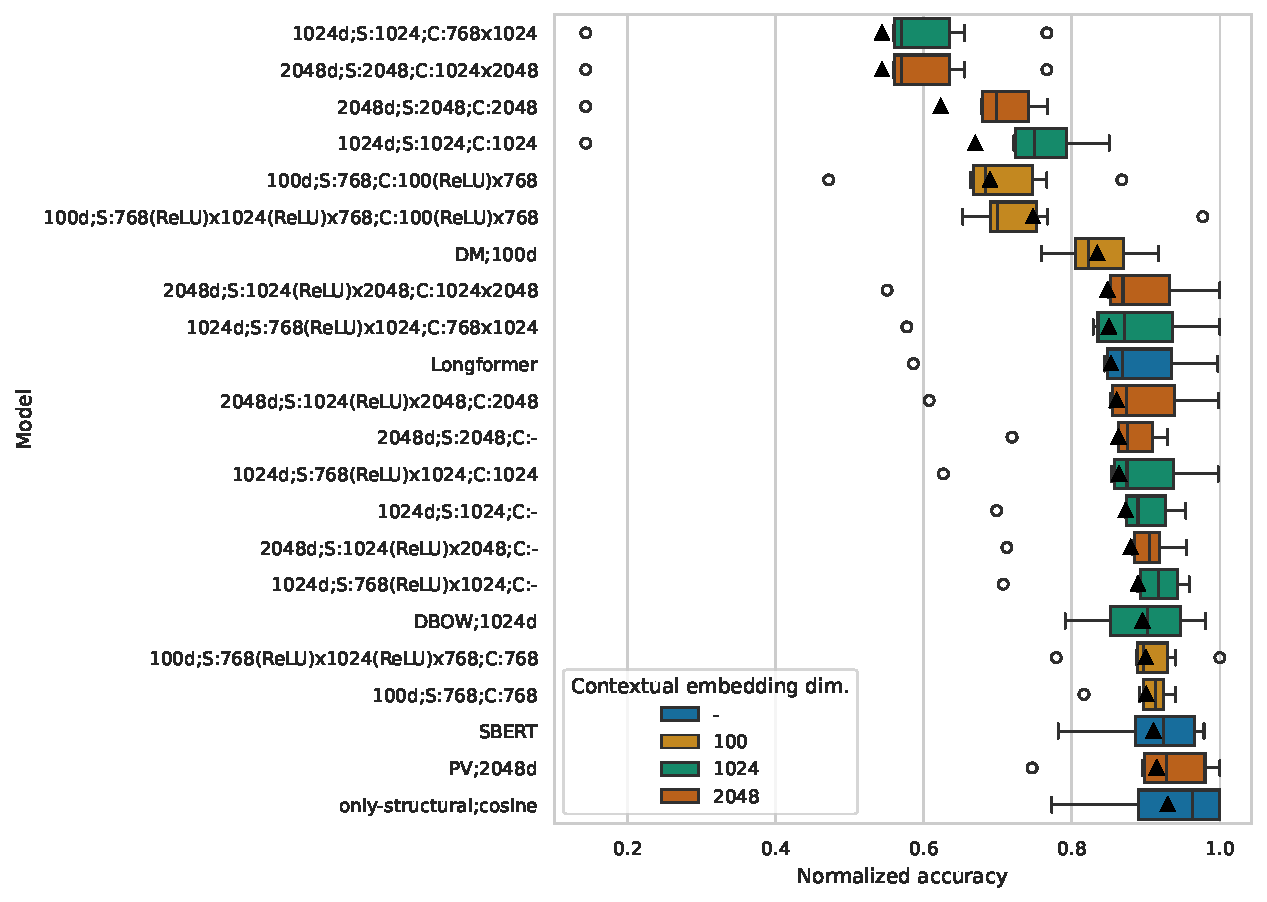
\includegraphics[width=\textwidth]{img/projections_contextual.pdf}

  \caption{Performances of student models trained with different projections
  and without structural loss. We compare the students to all the relevant
  teachers, Longformer, and \Model{only-structural;cosine}.}

  \label{fig:projections_contextual}

\end{figure}

\subsubsection{Contextual projection with cosine structural
loss}\label{section:projections_cos}

We now search for the best-performing projections while simultaneously using
cosine structural loss. The training is a bit
more complex than in the previous section as here the student should distill two qualities, each from a
different teacher. So, even though the student and contextual
projections still behave equally, they may cause different outcomes.

We list all the tested projections in
Table~\ref{table:cos_contextual_projections}. We add stronger projections
while discarding some of the less successful projections from the previous
section. We again train the student models on the first 15k documents of
\Dataset{val-500k} and present the performance of the trained student models in
Figure~\ref{fig:cos_projections_contextual}. The projection variants differ less than in the case of the student models trained without structural loss.
The cosine structural loss boosts the models' performance and lessens the
negative impact of a poor projection. As a consequence, almost all of the
student models surpass all baselines. The best-performing projections are much
larger compared to the best projections trained without any structural loss.
This seems logical, as the added structural loss puts more pressure on the
student, and so the contextual loss needs to give the model more freedom in
order to avoid conflict between the losses, which would slow down the training.
With the larger projections, we were able to surpass
\Model{only-structural;cosine}. This shows that, with the right projections, the student model benefits from both losses being used during
training. Even if the performance gain is not huge, we conclude that the
contextual and structural embeddings complement each other.

\begin{table}
  \centering
  \footnotesize

  \begin{subtable}{\textwidth}
    \centering
    \begin{tabular}{lr}
      \toprule
        & Contextual teacher's embedding dimension \\
        \cline{2-2} \\
        Projection & 100 \\
      \midrule
        Student & \Proj{768(ReLU)x1024(ReLU)x768}  \\
        \multirow[t]{2}*{Contextual} & \Proj{100(ReLU)x768}  \\
        & \Proj{768} \\
      \bottomrule
    \end{tabular}
    \caption{100-dimensional contextual teacher}
  \end{subtable}
  \medskip

  \begin{subtable}{\textwidth}
    \centering
    \begin{tabular}{lrr}
      \toprule
        & \multicolumn{2}{c}{Contextual teacher's embedding dimension} \\
        \cline{2-3} \\
        Projection & 1024 & 2048 \\
      \midrule
        Student &  \Proj{768(ReLU)x1024} & \Proj{1024(ReLU)x2048} \\
        \multirow[t]{2}*{Contextual} &  \Proj{1024} & \Proj{2048} \\
        & - & - \\
      \midrule
        Student & \Proj{768(ReLU)x4096(ReLU)x1024} & \Proj{768(ReLU)x4096(ReLU)x2048} \\
        \multirow[t]{3}*{Contextual} & \Proj{768(ReLU)x1024} & \Proj{2048(ReLU)x2048} \\
        & \Proj{1024} & \Proj{2048} \\
        & - & - \\
      \bottomrule
    \end{tabular}

    \caption{1024 and 2048-dimensional contextual teachers}

  \end{subtable}

  \caption{All tested variants of projections with contextual loss and cosine
  structural loss. For a given contextual teacher, we delimit each group of
  projections by a horizontal line. We grid search all variants within each
  group. This results in 12 combinations of projections.}

  \label{table:cos_contextual_projections}
\end{table}

\begin{figure}

  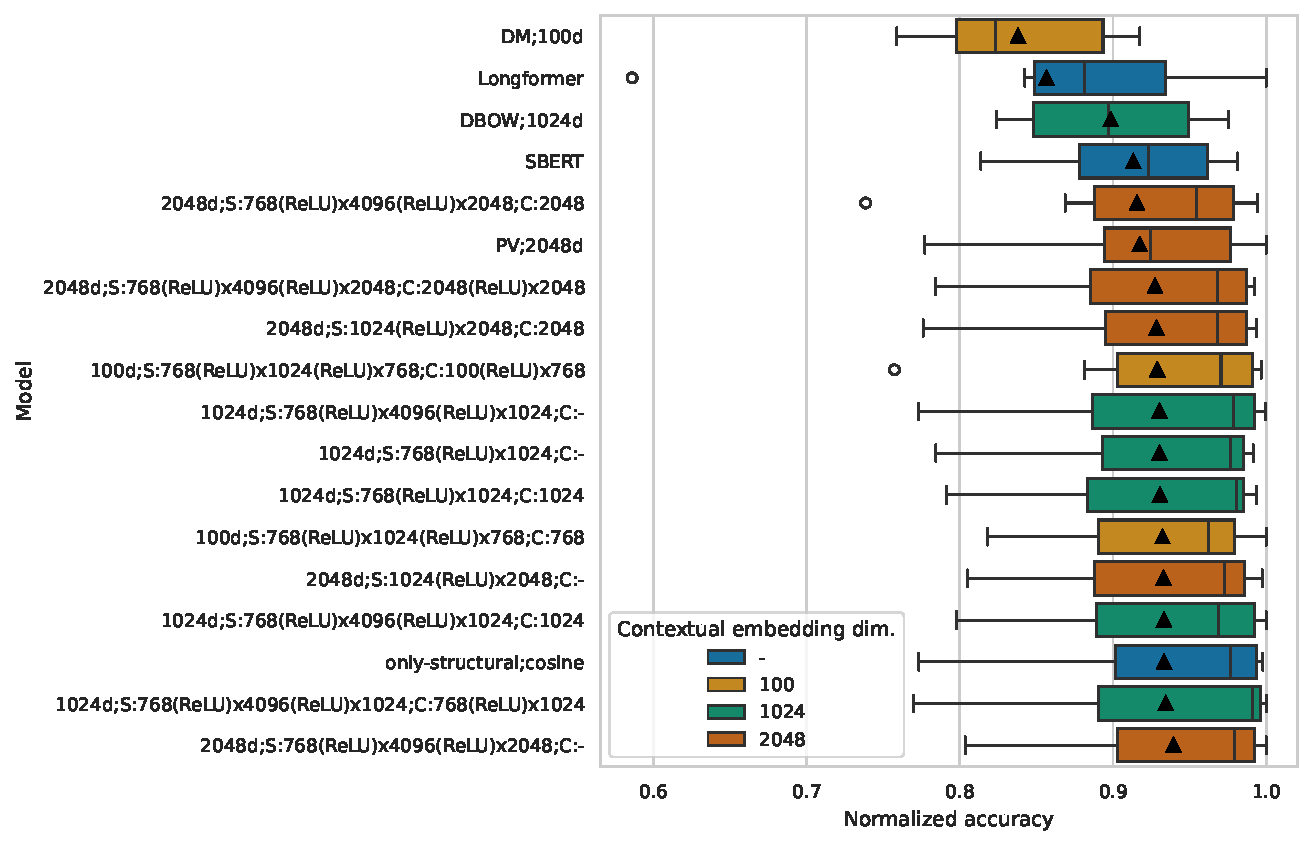
\includegraphics[width=\textwidth]{img/projections_contextual_cos.pdf}

  \caption{Performance of student models trained with contextual and cosine
  structural loss on validation tasks. We compare the student models to all
  relevant teachers, Longformer and \Model{only-structural;cosine}.}

  \label{fig:cos_projections_contextual}

\end{figure}

\subsubsection{Contextual projection with max-marginals MSE structural
loss}\label{section:projections_mm_mse}

We also search for optimal projections when simultaneously training with the
max-marginals MSE loss. As we show in
Section~\ref{section:composite_analysis}, max-marginals MSE structural loss
goes against the goal of our student-teacher training. Yet, it surpassed all the
composite and simple structural losses. We continue experimenting with it
here to see how the student reacts to different configurations of the contextual loss.

We present all the tested projection variants in
Table~\ref{table:mm_mse_contextual_projections}. We include successful
projections from the previous section and add stronger contextual projections as
they perform surprisingly well in this context. Same as before, we train all
student models on the first 15k documents from \Dataset{val-500k} and compare
their performance to all relevant teachers, Longformer, and
\Model{only-structural;mm-MSE}. We present the model's performances in
Figure~\ref{fig:mm_mse_contextual_projections}. As with the cosine
structural loss, max-marginals MSE loss boosts the students' performances.
Consequently, the student's performances are not as dependent on
the projections as those of students trained without
structural loss. Contrary to what we witness in previous experiments, stronger
contextual projections perform very well overall. This shows that max-marginals MSE loss exerts so much pressure on the student's embedding the projections
need to be even stronger than in the case of cosine structural loss. Again, the max-marginals MSE structural loss does not quite correspond with our
training technique. As a consequence, despite testing even more projections
than in the case of cosine structural loss, we fail to find projections with
which the student would benefit from both contextual and max-marginals MSE
structural losses used during training.

\begin{table}
  \centering
  \footnotesize

  \begin{subtable}{\textwidth}
    \centering
    \begin{tabular}{lr}
      \toprule
      % TODO: name the same in the chart or rename it here
        & Contextual teacher's embedding dimension \\
        \cline{2-2} \\
        Projection & 100 \\
      \midrule
        \multirow[t]{2}*{Student} & \Proj{768(ReLU)x1024(ReLU)x768}  \\
        & \Proj{768} \\
        \multirow[t]{2}*{Contextual} & \Proj{100(ReLU)x768}  \\
        & \Proj{768} \\
      \bottomrule
    \end{tabular}
    \caption{100-dimensional contextual teacher}
  \end{subtable}
  \medskip

  \begin{subtable}{\textwidth}
    \centering
    \begin{tabular}{lrr}
      \toprule
        & \multicolumn{2}{c}{Contextual teacher's embedding dimension} \\
        \cline{2-3} \\
        Projection & 1024 & 2048 \\
      \midrule
        Student &  \Proj{768(ReLU)x1024} & \Proj{1024(ReLU)x2048} \\
        \multirow[t]{3}*{Contextual} & \Proj{768x1024} & \Proj{1024x2048} \\
        & \Proj{1024} & \Proj{2048} \\
        & - & - \\
      \midrule
        Student & \Proj{768(ReLU)x4096(ReLU)x1024} & \Proj{768(ReLU)x4096(ReLU)x2048} \\
        \multirow[t]{3}*{Contextual} & \Proj{1024(ReLU)x1024} & \Proj{2048(ReLU)x2048} \\
        & \Proj{768(ReLU)x1024} & - \\
      \bottomrule
    \end{tabular}

    \caption{1024 and 2048-dimensional contextual teachers}

  \end{subtable}

  \caption{All variants of projections tested with
  max-marginals MSE structural loss. For a given contextual teacher, we delimit
  each group of projections by a horizontal line. We grid-search all variants
  within a group. This results in 14 combinations in total.}

  \label{table:mm_mse_contextual_projections}
\end{table}

\begin{figure}

  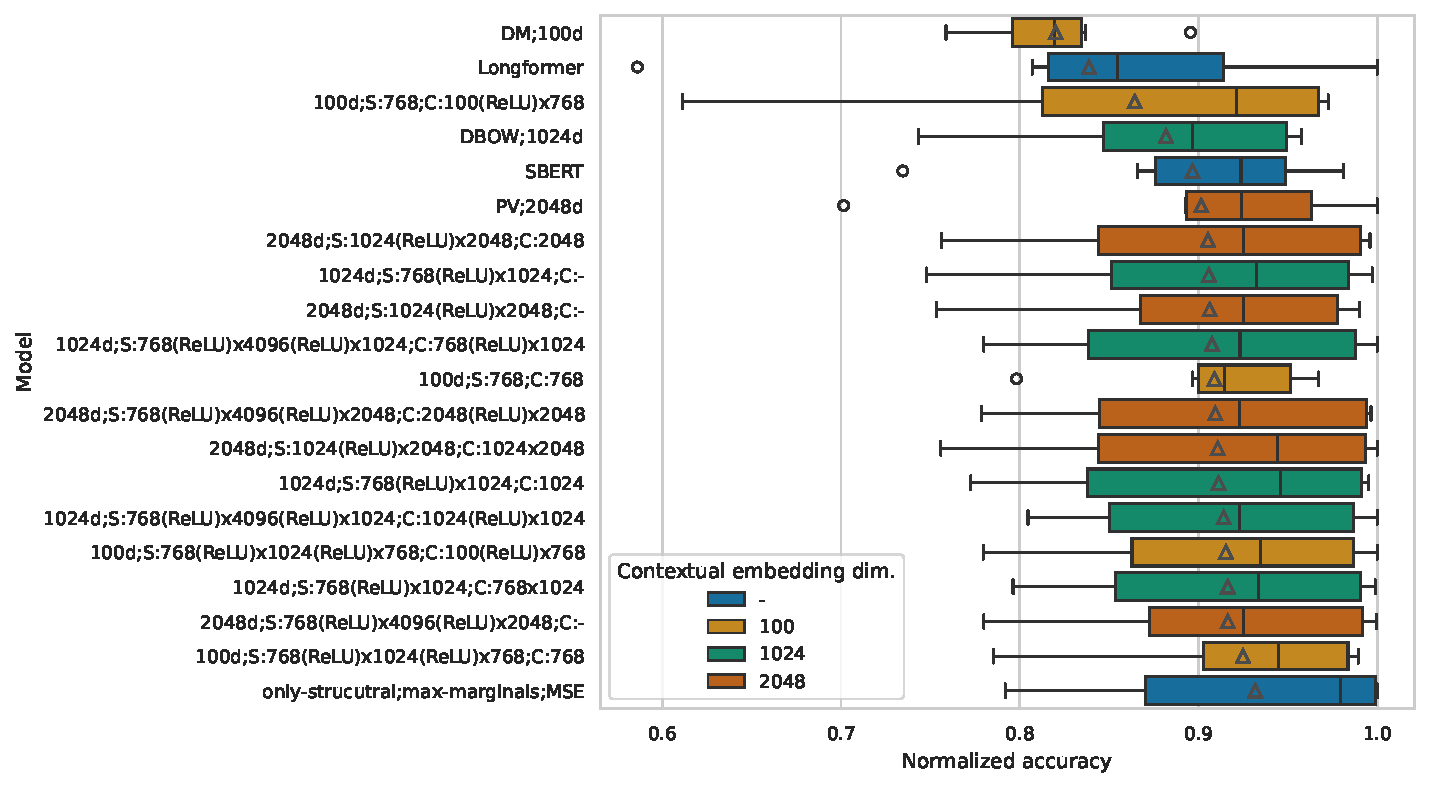
\includegraphics[width=\textwidth]{img/projections_contextual_mm_mse.pdf}

  \caption{Performance of student models trained with contextual and
  max-marginals MSE structural loss on validation tasks. We compare the student
  models to all relevant teachers, Longformer and
  \Model{only-structural;mm-MSE}.}

  \label{fig:mm_mse_contextual_projections}

\end{figure}

\subsection{Weighting of structural and contextual
loss}\label{section:weighting_experiments}

The final loss is a weighted sum of the contextual and the structural loss. In
this section, we explore two weighting mechanisms. First, we assign static
weights to each loss. Second, we combine the static weights with dynamic
masking of inputs based on their length. As the structural teacher has limited
context length, its embedding only reflects the information in the first 384
tokens. We use dynamic masking to train the student only on those inputs, which
the structural teacher encodes whole. Therefore, in theory, the structural loss
should be more reliable. To summarize, we grid-search two parameters: \texttt{max\_structural\_len} and $\lambda$.
\texttt{max\_structural\_len} determines which inputs' structural loss we
mask out. $\lambda$ is the static weight used for unmasked inputs to
balance the importance of the structural and contextual loss. For clarity, we
include a Python-like pseudocode of the weighting algorithm in
Listing~\ref{lst:weighting}.

\begin{figure}
\begin{lstlisting}[caption=Python-like pseudocode of weighting algorithm.,label={lst:weighting}]
length_mask @\High{symbols}=@ torch.@\High{functions}ones@(batch_size)
if max_structural_len is not @\High{types}None\High{symbols}:@
  length_mask @\High{symbols}=@ lengths @\High{symbols}<=@ max_structural_len
lams @\High{symbols}=@ torch.@\High{functions}zeros@(batch_size).@\High{functions}fill\verb|_|@(@$\lambda$@)
lams @\High{symbols}*=@ length_mask

# For each loss we expect shape (batch_size,)
structural_loss @\High{symbols}=@ @\High{functions}\verb|structural_loss_fn|@(@\ldots@, mask=length_mask)
contextual_loss @\High{symbols}=@ @\ldots@

loss @\High{symbols}=@ structural_loss @\High{symbols}*@ lams @\High{symbols}+@ contextual_loss @\High{symbols}*@ (@\High{constants}1@ @\High{symbols}-@ lams)
loss @\High{symbols}=@ torch.@\High{functions}mean@(loss)
\end{lstlisting}
\end{figure}

In previous experiments, we weight the losses less intrusively. We do not
mask out structural loss and sum the two losses. The advantage
of this approach is that it does not reduce gradients. However, we
lose control over the mix of the two losses. Even if the losses are not
weighted, we see this as another variant of obtaining the final loss and label
it as \Model{no-weighting}. We label all other weighting variants with the used
\texttt{max\_structural\_len} and $\lambda$ separated by a semicolon.

We consider two structural losses: cosine and max-marginals MSE. For each
structural loss, we take the best-performing contextual loss from the previous
section and try all combinations of weighting hyperparameters' values we list
in Table~\ref{table:weighting_variants}. We train a student model with each
weighting variant on the first 15k documents from \Dataset{val-500k}.

\begin{table}
  \centering
  \footnotesize
  \begin{tabular}{cc}
    \toprule
    \texttt{max\_structural\_len} & $\lambda$ \\
    \midrule
    384 & 0.95 \\
    None & 0.8 \\
    & 0.5 \\
    & 0.2 \\
    \bottomrule
  \end{tabular}

  \caption{Tested weighting hyperparameters' values. We experiment with several
  static weightings $\lambda$ with or without dynamic masking of structural
  losses for inputs longer than 385 tokens.}

  \label{table:weighting_variants}

\end{table}

\subsubsection{Weighting a contextual and the cosine structural loss}

We experiment with contextual loss and cosine structural loss in
Section~\ref{section:projections_cos}. In this context, the best performing
projections are \Proj{S:768(ReLU)x4096(ReLU)x2048;C:-} in combination with
\Model{PV;2048d} contextual teacher. So, we perform the weighting
experiments with the same projections and contextual teacher.

We compare the students' performances to the relevant baselines, the
\Model{no\-weighting} variant and \Model{only-structural;cosine}. We present
all the models' performances in Figure~\ref{fig:cos_weighting}. All the
weighting variants surpass all baselines. Interestingly, even if the weighting
is set significantly toward one side, such as \Model{None;$\lambda$=0.95} or
\Model{384;$\lambda$=0.2}, the student model can surpass the other
teacher. Therefore, the student can use the information provided by
either teacher to surpass the other one. More importantly, the best weighting
variants that beat \Model{only-structural;cosine} are more cautious with the
structural loss. They either mask it for longer documents or give it a smaller
weight. Consequently, forcing the student model to distill
embedding that captures only a partial part of its input confuses it, thereby hurting its performance.

\begin{figure}
  \centering
  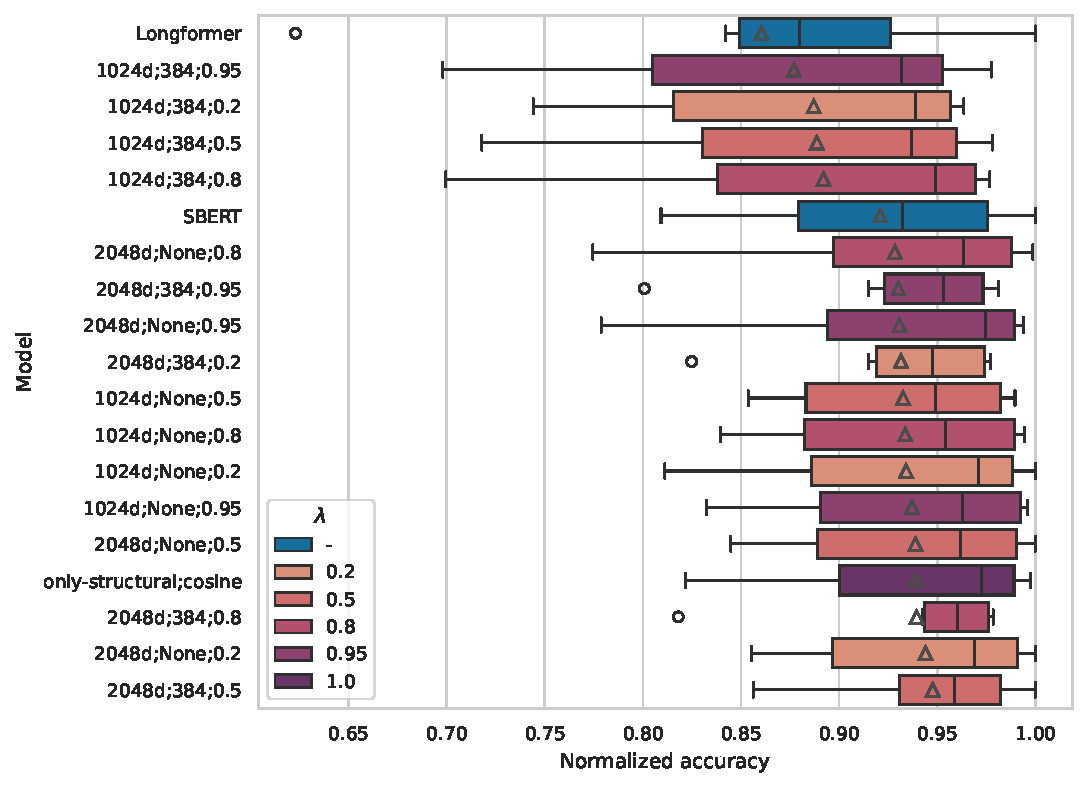
\includegraphics[width=0.85\textwidth]{img/cos_weighting.pdf}

  \caption{Performances of all weighting variants trained with cosine
  structural loss. We compare the student models to Longformer, SBERT, and
  \Model{only-structural;cosine}.}

  \label{fig:cos_weighting}

\end{figure}

We highlight the difference in performance between \Model{None;$\lambda$=0.5}
and \Model{no-weighting}. These models' losses are the same, except
that \Model{None;$\lambda$=0.5} effectively halves all loss gradients. This results in a
noticeable drop in performance. However, even with the gradients being halved,
\Model{384;$\lambda$=0.5} beats \Model{no-weighting} variant. This further
emphasizes the importance of masking out structural loss for long inputs.

\subsubsection{Weighting a contextual and the max-marginals MSE structural
loss}

As we ascertain in Section~\ref{section:projections_mm_mse}, with max-marginals
MSE structural loss, the projections that perform the best are
\Proj{S:768(ReLU)x1024(ReLU)x768;C:768} with \Model{DM;100d} contextual
teacher. However, even with this projection and contextual teacher, the model
performs worse than \Model{only-structural;mm-MSE}. Nevertheless, we continue
experimenting with the given projections and contextual teacher to see if we
can improve the model by different weightings of the contextual and
max-marginals MSE structural losses and perhaps show that with smaller
contextual weight, the model may benefit from the contextual loss.

Again, we compare the weighting variants to Longformer, SBERT, \Model{DM;100d},
and \Model{only-structural;mm-MSE}. We display the models' performances in
Figure~\ref{fig:mm_mse_weighting}. In the case of max-marginals MSE, masking
out some inputs' structural loss significantly hurts performance. As the loss is masked for some inputs, the number of negatives for
each input effectively decreases. As we discuss in
Section~\ref{section:composite_analysis}, the performance of max-marginals MSE comes from different inputs having distant embeddings. By masking out some inputs, we are hiding long documents, whose embedding may end up close to some embeddings of shorter documents, which has the loss seen and adjusted. These neighboring embeddings of different inputs would ultimately hurt the model's performance. Note that the weighting variants
with higher $\lambda$ suffer from this effect considerably more.

Even without any masking, the different loss weightings fail to improve the
score of \Model{only-structural;mm-MSE}. When comparing the two nearly
identical weighting variants \Model{no-weighting} and
\Model{None;$\lambda$=0.5}, we see that \Model{no-weighting}, which trains
with gradients twice as big, is worse. Such results suggest that, with the
max-marginals MSE structural loss, the more we train with the contextual loss,
the worse the model will be. Ultimately, this confirms the conclusions
from Section~\ref{section:projections_mm_mse}, where we do not find any
projections with which the model would benefit from a contextual loss.

\begin{figure}

  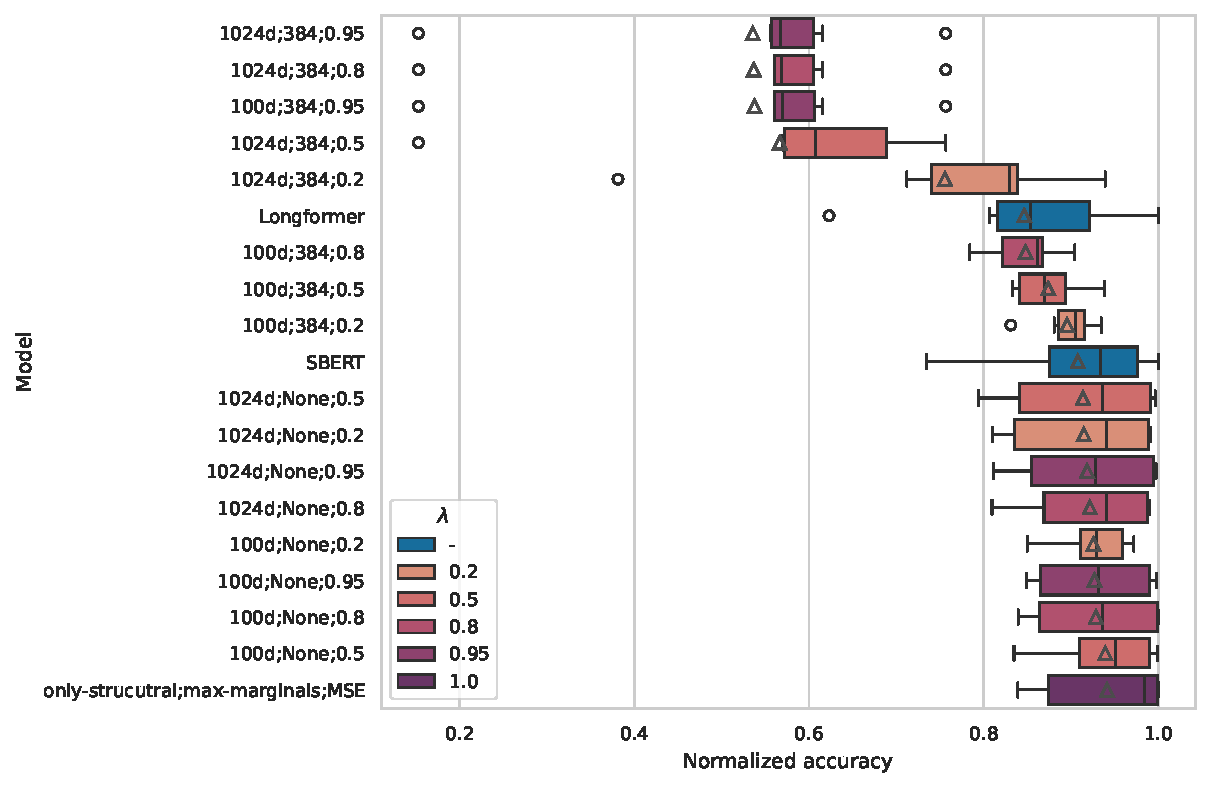
\includegraphics[width=0.9\textwidth]{img/mm_mse_weighting.pdf}

  \caption{Performances of all weighting variants for max-marginals MSE
  structural loss. We compare the students to Longformer, SBERT,
  \Model{DM;100d} contextual teacher and \Model{only-structural;mm-MSE}.}

  \label{fig:mm_mse_weighting}

\end{figure}

\section{Summary}\label{section:experiments_summary}

After an extensive experimentation with our teacher-student training method, we
summarize what we test, but mainly how we interpret the results and what
conclusions we draw from them.

First, in Section~\ref{section:structural_loss}, we experiment with simple and
composite structural losses. While simple losses focus only on the similarity
between the student's and the corresponding teacher's embedding, composite
losses also take advantage of the in-batch teacher's embedding of different
inputs. Cosine is the best performing simple structural loss, surpassing even
SBERT. These results show that the combination of Longformer's architecture and
distillation of SBERT's embeddings can boost the student's performance even
above the level of the structural teacher. However, cosine performs worse than
the best composite loss, which is max-marginals with MSE. As we show in
Section~\ref{section:composite_analysis}, max-marginals MSE losses use SBERT's
embeddings to increase the distance between student's embeddings of distinct
inputs. Thus, we conclude that distillation of a certain quality from a student
model may be less effective than increasing the difference between distinct
input embeddings.

In Section~\ref{section:structural_and_contextual}, we try to leverage the
contextual loss to improve the models trained with just the cosine or
max-marginals MSE structural loss. After finding promising training
hyperparameters for Paragraph Vector, we show that the contextual loss alone
can improve Longformer's results. Yet, it cannot surpass SBERT or the student
models trained with just the structural loss. This demonstrates that the
contextual teacher is more important to the student's performance in our
setting than the contextual teacher. We also find the optimal contextual loss
for cosine and max-marginals MSE loss. In the case of cosine structural loss,
the student can benefit from both the contextual and the structural loss if the
contextual loss is less exact, which gives the student enough freedom. With the
max-marginals MSE structural loss, the contextual loss needs to be far less
strict, and even then, it fails to improve the student model trained with just
the structural loss. We also try more involved ways to weigh the contextual and
the structural loss. In the case of max-marginals MSE structural loss, we find
that even with a significant emphasis on the structural loss, the student model
suffers from both the contextual loss and the max-marginals MSE loss used
simultaneously. So, we conclude that max-marginals MSE is incompatible with our
training method. On the other hand, with cosine structural loss, the student
model behaves intuitively. It prefers an equal balance of the structural and
the contextual loss, where the structural loss is used only for inputs the
structural teacher can encode whole.

To summarize, we have two configurations  of our training method, which result
in promising models. We label these models according to their structural loss
as \Model{cosine} and \Model{mm-MSE}. \Model{cosine} uses structural and
contextual loss to distill the qualities of the two teachers' embeddings, as
described in Chapter~\ref{chapter:training_method}. Even though \Model{mm-MSE}
originates from our method, its training fulfills a different objective. It
only uses a composite structural loss to move the embeddings of distinct inputs
further apart instead of moving them closer to their corresponding SBERT
embeddings. As we present in Figure~\ref{fig:experiments_final_comparison},
\Model{mm-MSE} beats \Model{cosine} in four out of six tasks.

\begin{figure}
    \centering
    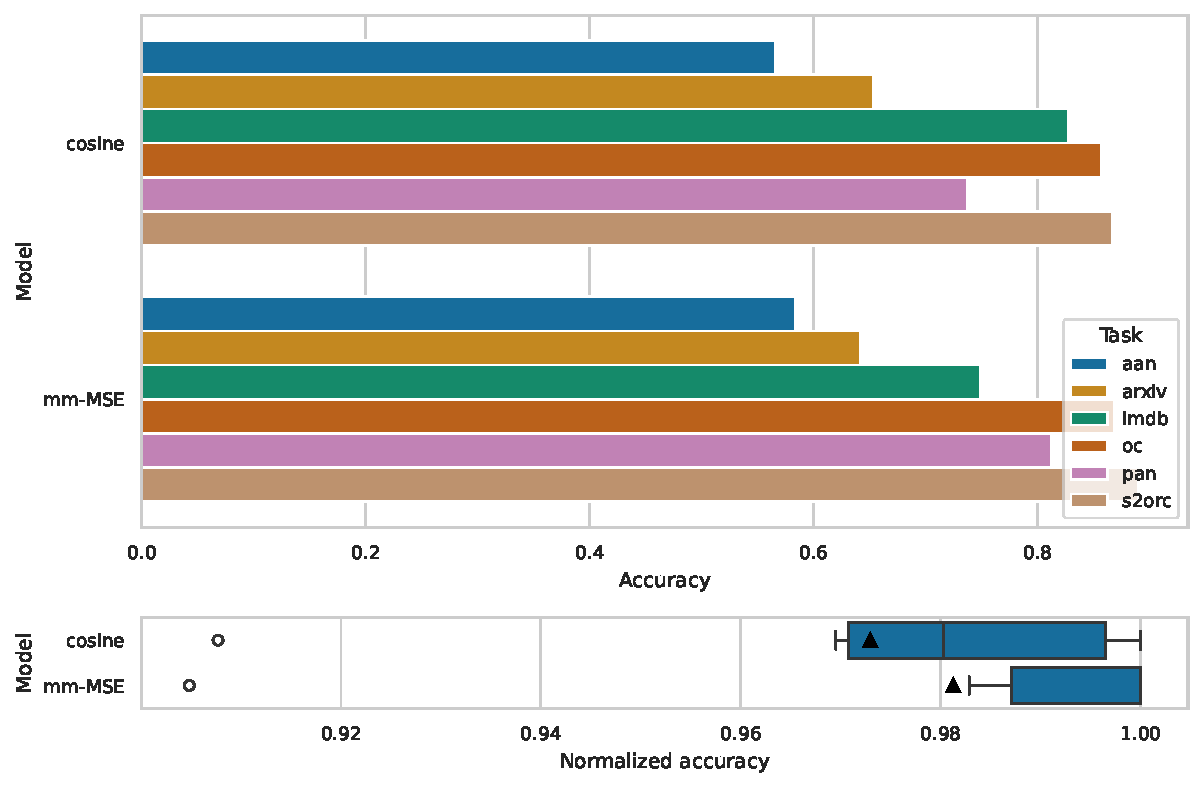
\includegraphics[width=\textwidth]{img/experiments_final_models.pdf}

    \caption{Performance of two final model variants on validation tasks.}

    \label{fig:experiments_final_comparison}

\end{figure}

\chapter{Evaluation}\label{chapter:evaluation}

In this chapter, we evaluate the most promising configurations of our training
method. We train three student models on 1M documents with the best-performing
hyperparameters from Chapter~\ref{chapter:experiments} to show the effects of
long training with our teacher-student method. We evaluate the student models
on six classification and two retrieval tasks. For classification tasks, we
consider three different limits on the amount of available supervised data. We
show the models' performances vary for different limits and thus highlight
the strengths and limitations of our training method.

\section{Student models}

We only evaluate the three best-performing variants of our training method from
Chapter~\ref{chapter:experiments}. We use the hyperparameters listed in Table~\ref{table:experiments_final_config}, however, as we train the student models and the contextual teachers on significantly
more data, we label the models differently. {\CosineStudent}
is trained with a balanced mix of contextual loss and cosine structural loss,
which is masked out for inputs longer than the structural teacher's maximum
context length. {\MSEStudent} is trained with an equal mixture of contextual
loss and a max-margin MSE structural loss. Finally, {\OnlyMSEStudent} is
trained only on the max-margin MSE structural loss. These models'
hyperparameters correspond to the configurations of
\Model{masked-cosine;$\lambda$=0.5}, \Model{mm-MSE;$\lambda$=0.5}, and
\Model{only-structural;mm-MSE} from Table~\ref{table:experiments_final_config},
respectively.

\subsection{Training data}

We compile our training corpus the same as \Dataset{val-500k}. We train the
student models only using Longformer's training data. Without any new training
data, the performance of our student model depends only on our training
method. Hence, the performances of the student models are proportional to our
training method's performance, which gives us an easy way to gauge the benefits of our training method.

Following Longformer's approach, we equally sample articles from the English
Wikipedia\footnote{\url{https://huggingface.co/datasets/wikipedia/viewer/20220301.en}}
and documents from the RealNews dataset \citep{zellers2019defending} that have
above 1200 Longformer's tokens. We label the resulting dataset as
\Dataset{train-1M} and display its statistics in
Table~\ref{table:train_data_stats}. \Dataset{train-1M} contains relatively long
documents. The average document has around 1300 tokens, and only 34\% of its
documents can fit into the maximum context length of a vanilla Transformer.
However, as we show in Figure~\ref{fig:train_data_dist}, most documents have
between 0 and 500 tokens or 1200 and 1700 tokens.

\begin{table}
    \centering
    \footnotesize
\begin{tabular}{lrr}
\toprule
Split & Train & Validation \\
\midrule
Documents & 1 000 000 & 30 000 \\
Tokens & 1.37e+09 & 4.15e+07 \\
Tokens per document & 1375$\pm$1738 & 1382$\pm$1697 \\
SBERT tokens over 384 & 71\% & 71\% \\
SBERT tokens over 512 & 66\% & 67\% \\
\bottomrule
\end{tabular}


    \caption{Statistics of \Dataset{train-1M}. For each split, we also show
    the percentage of documents with the number of SBERT tokens above the given
    threshold.}

    \label{table:train_data_stats}

\end{table}

\begin{figure}
    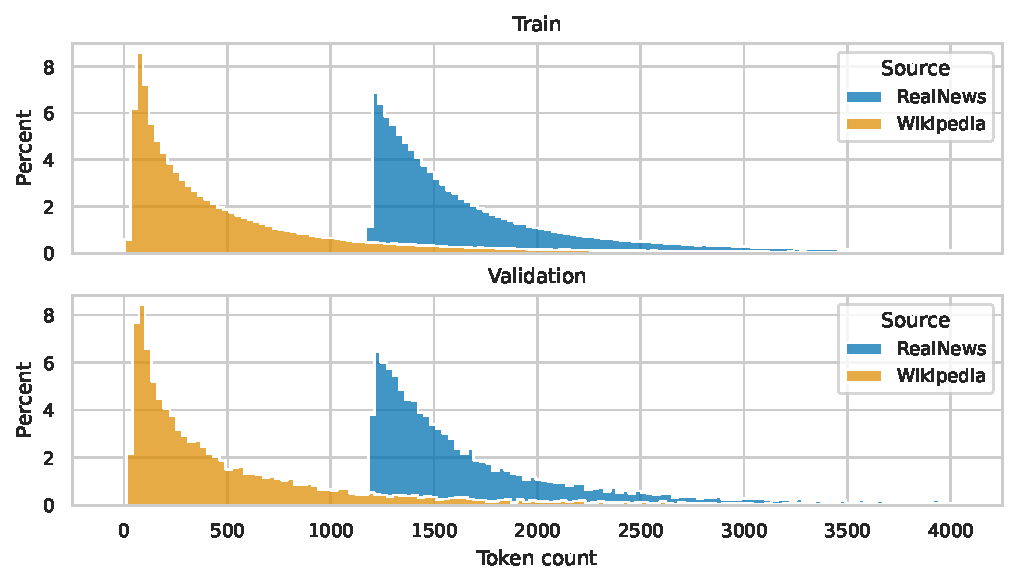
\includegraphics[width=\textwidth]{./img/train_data_dist.pdf}

    \caption{Distribution of the number of Longformer tokens per document in
    \Dataset{train-1M}.}

    \label{fig:train_data_dist}
\end{figure}


\subsection{Training of contextual teachers}

Two of our student models use a contextual teacher. To showcase the full
potential of our training method, we train the contextual teachers anew and
with much more data than in the previous chapter. {\CosineStudent} uses a
2048-dimensional Paragraph Vector \citep{le2014distributed} composed of
Distributed Memory and Distributed Bag of Words models. {\MSEStudent} uses only
a 100-dimensional Distributed Memory model. These contextual teachers correspond to \Model{PV;2048d} and \Model{DM;100d} from Section~\ref{section:pv_training} respectively.

We compile the contextual teacher's training dataset in the same manner as
\Dataset{train-1M}. Since the contextual teachers' training
data also becomes the student's training data, we restrict it to Longformer's training data for the
reasons we mention in the previous section. However, as PV is a significantly
smaller model than our student model, we can afford to train it with
substantially more data. We use all available data from RealNews articles and
an equal amount of Wikipedia documents. The resulting dataset has 8.3 million
documents. We label the trained 100-dimensional and 2048-dimensional teachers
\Model{DM} and \Model{PV}. To keep the models' memory footprint manageable, we
restrict \Model{DM}'s vocabulary to $6\times 10^7$ words and \Model{PV}'s
vocabulary to $1.2\times 10^7$ words. With these limitations, the models take
up approximately 96GB and 124GB of memory during prediction.

\subsection{Training of student models}

Finally, we train the student models with the newly trained contextual teachers.
We train on \Dataset{train-1M} for one epoch with hyperparameters listed in
Table~\ref{table:final_student_train_params}. Thanks to the student's efficient
self-attention, the models take up only 12GB of VRAM during training. We train
the models on an NVIDIA A100 GPU card for approximately 30 hours.

\begin{table}
  \centering
  \footnotesize

  \begin{tabular}{l c}
    \toprule
    Parameter & Value \\
    \midrule
    Batch size & 6 \\
    Weight decay & 0.1 \\
    Learning rate & 3e-5 \\
    Learning rate decay & Cosine \\
    Maximum gradient norm & 1.0 \\
    Optimizer & AdamW \\
    Gradient accumulation steps & 10 \\
    Warmup update steps & 500\\
    Gradient checkpointing & Yes \\
    Mixed-precision training & Yes \\
    \bottomrule
  \end{tabular}

  \caption{Hyperparameters used for training all three student models:
  {\CosineStudent}, {\MSEStudent}, and {\OnlyMSEStudent}.}

  \label{table:final_student_train_params}

\end{table}

\section{Evaluation tasks}

We thoroughly evaluate the student models using eight diverse tasks. We
select six classification tasks that cover citation prediction, plagiarism
detection, sentiment, and topic classification. We also include two retrieval
tasks from distinct domains.

We present an overview of the selected classification tasks in
Table~\ref{table:eval_cls_tasks_overview}. Besides ordinary classification
tasks, we also include classifications of document pairs. In these tasks,
the classifier bases its prediction on the comparison of two documents, or in
our case,  their two embeddings. As can be seen from
Table~\ref{table:evaluation_tasks_stats}, the amount of the tasks' finetuning
and evaluation data ranges. This becomes particularly important in
Section~\ref{section:eval_cls_tasks}, where we evaluate the student models
while limiting the tasks' training data to different amounts.

\begin{table}
  \footnotesize
  \centering

  \begin{tabular}{llrrr}
      \toprule
      \multicolumn{3}{c}{} & \multicolumn{2}{c}{Class percentage $\sigma$} \\
      \cline{4-5}
      Dataset & Inputs & Classes & Train & Test \\
      \midrule
      \Task{arxiv} & documents & 11 & 1.25 & 1.30 \\
      \Task{imdb} & documents & 2 & 0.00 & 0.00 \\
      \Task{aan} & pairs of documents & 2 & 1.50 & 0.77 \\
      \Task{oc} & pairs of documents & 2 & 0.07 & 0.34 \\
      \Task{pan} & pairs of documents & 2 & 0.00 & 0.00 \\
      \Task{s2orc} & pairs of documents & 2 & 0.09 & 0.33 \\
      \bottomrule
  \end{tabular}

  \caption{Overview of the classification tasks. For each task, we include the
  type of input classified. The class distributions for all tasks are on
  average balanced, thus we show only the standard deviation of class
  percentages.}

  \label{table:eval_cls_tasks_overview}

\end{table}

\begin{table}
  \footnotesize
  \centering
    \begin{tabular}{llrrr}
        \toprule
        & & & \multicolumn{2}{c}{SBERT tokens} \\
        \cline{4-5}
        Dataset & Split & Documents & Over 384 & Over 512 \\
        \midrule
        \multirow[c]{2}{*}{\Task{arxiv}} & Train & 28 388 & 100\% & 100\% \\
        & Test & 2 500 & 100\% & 100\% \\
        \cline{1-5}
        \multirow[c]{2}{*}{\Task{imdb}} & Train & 25 000 & 25\% & 15\% \\
        & Test & 25 000 & 24\% & 14\% \\
        \cline{1-5}
        \multirow[c]{2}{*}{\Task{aan}} & Train & 106 592 & 0\% & 0\% \\
        & Test & 13 324 & 0\% & 0\% \\
        \cline{1-5}
        \multirow[c]{2}{*}{\Task{oc}} & Train & 240 000 & 12\% & 1\% \\
        & Test & 30 000 & 12\% & 1\% \\
        \cline{1-5}
        \multirow[c]{2}{*}{\Task{pan}} & Train & 17 968 & 70\% & 59\% \\
        & Test & 2 906 & 61\% & 47\% \\
        \cline{1-5}
        \multirow[c]{2}{*}{\Task{s2orc}} & Train & 152 000 & 33\% & 19\% \\
        & Test & 19 000 & 33\% & 18\% \\
        \cline{1-5}
        \bottomrule
    \end{tabular}

    \caption{Statistics of the classification tasks. We
    include the percentage of documents with SBERT tokens above a given
    threshold for each task and split.}

    \label{table:evaluation_tasks_stats}

\end{table}

We present an overview of the retrieval tasks in
Table~\ref{table:eval_sims_tasks}. These tasks do not have any finetuning data
and test only the proximity of embeddings of similar documents. Both tasks have
around 90 source articles, each with around eight similar target articles.
However, \Task{games} has substantially more documents.

\begin{table}
  \centering
  \footnotesize
  \begin{tabular}{lrrrrr}
    \toprule
    & & & & \multicolumn{2}{c}{SBERT tokens} \\
    \cline{5-6}
    Dataset & Documents & Sources & Targets per source & Over 384 & Over 512 \\
    \midrule
    \Task{wines} & 1 662 & 89 & 8.92$\pm$1.23 & 100\% & 90\% \\
    \Task{games} & 21 228 & 88 & 8.74$\pm$2.35 & 100\% & 92\% \\
    \bottomrule
  \end{tabular}

  \caption{Statistics of our similarity-based evaluation tasks. Each dataset
  has around 90 source documents, each similar to around nine target documents.
  We also include the percentage of documents with SBERT tokens above the given
  threshold.}

  \label{table:eval_sims_tasks}

\end{table}

We pay special attention to the lengths of documents contained in the datasets
and try to cover a span of lengths as large as possible. However, high-quality long document datasets are very rare due to their annotation's high complexity
and cost. Often, a dataset is said to be composed of documents, but it contains
only shorter pieces of text, such as abstracts. So, we include only one dataset
containing very long documents. As Figure~\ref{fig:eval_tasks_length_dist}
shows, the tasks arguably focus more on documents up to around 1024 tokens.
Nonetheless, as we show in
Tables~\ref{table:evaluation_tasks_stats}~and~\ref{table:eval_sims_tasks} the
tasks still contain a considerable number of documents longer than the maximum
context of our structural teacher.

\begin{figure}

    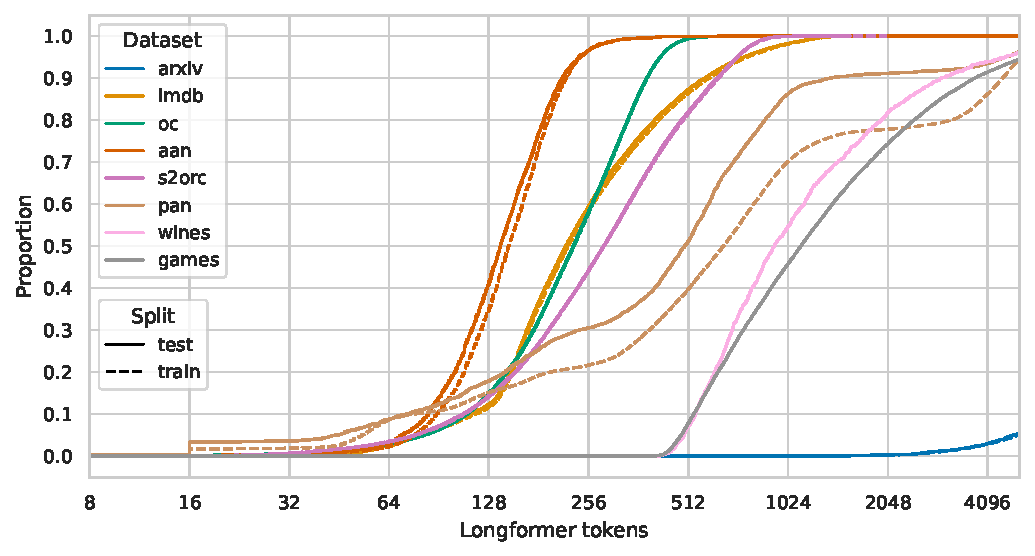
\includegraphics[width=\textwidth]{./img/eval_tasks_token_ecdf.pdf}

    \caption{Estimated cumulative length distribution of the number of
    Longformer tokens in a document.}

    \label{fig:eval_tasks_length_dist}
\end{figure}

\subsection{Tasks' description}

\paragraph{IMDB movie reviews.} The IMDB dataset~\citep{maas2011learning}
(denoted as \Task{imdb}) is a binary classification dataset frequently used to
evaluate long-context NLP models~\citep{zaheer2020big, beltagy2020longformer,
le2014distributed}. The dataset consists of movie reviews, each with an
associated rating on a 10-point scale. The reviews that rated the movie with 7
points or higher are classified as positive, and reviews with less than 4
points are classified as negative. There can be up to 30 reviews for each
movie, and the test set contains a disjoint set of movies. Along with the train
and test splits, the dataset contains an unsupervised split without rating or
class labels.

\paragraph{Arxiv papers.} Arxiv papers~\citep{arxiv_papers} (denoted as
\Task{arxiv}) is a collection of papers from ArXiv (\url{arxiv.org}),
an online archive of scholarly papers. Each paper contains its text truncated
to 10000 words but spanning at least 1000 words. The papers are classified into
11 groups based on the scientific field of the given paper. Since each paper
can be associated with several scientific fields, a small portion of the
documents ($\approx$~3.1\%) appear more than once but with different labels.
The scientific fields cover mainly fields of Computer science, such as
Artificial intelligence or Data structures, but also fields connected with
Mathematics, such as Group theory or Statistics theory.

\paragraph{ACL Anthology Network Corpus citations.} The ACL Anthology Network
Corpus citations dataset~\citep{zhou2020multilevel} (denoted as \Task{aan}) is
a citation prediction dataset. Each example in the dataset contains a pair of
paper abstracts and is classified as positive if the first document cites the
second one or negative if it does not. The dataset is compiled from the ACL
Anthology Network Corpus~\citep{radev2013acl}, where each source paper creates
positive pairs with all cited papers and a negative pair with one other randomly
sampled non-cited paper.

\paragraph{Semantic Scholar Open Corpus citations.} The Semantic Scholar Open
Corpus citations dataset~\citep{zhou2020multilevel} (denoted as \Task{oc}) is
also a citation prediction dataset in the same format as \Task{aan}. As the
dataset name suggests, it was compiled from the Semantic Scholar Open
Corpus~\citep{bhagavatula2018content}. In this dataset, only a single positive
pair is generated for each source paper, resulting in a much higher count of
unique papers compared to \Task{aan}.

\paragraph{PAN plagiarism detection.} The next classification dataset is the
PAN plagiarism detection dataset~\citep{zhou2020multilevel} (denoted as
\Task{pan}). It was constructed from PAN plagiarism alignment
task~\citep{potthast2013overview}, which is a collection of pairs of web
documents, where the sections relevant to plagiarism are humanly annotated both
in the source as well as in the suspicious document. \Task{pan} is a binary
classification task where each document pair is classified as positive or
negative. Positive inputs contain the source's plagiarised section, with a part of
the suspicious document containing the corresponding plagiarised section.
Negative pairs are constructed from the positives by replacing the source's
segment with a different part of the same document that is not annotated as being
plagiarised.

\paragraph{Semantic Scholar Open Research Corpus citations.} The Semantic
Scholar Open Research Corpus citations dataset~\citep{zhou2020multilevel}
(denoted as \Task{s2orc}) is our third and final citation prediction dataset.
The source of this dataset is the Semantic Scholar Open Research
Corpus~\citep{lo2019s2orc}, where each paper is divided into sections
connected via links to the papers cited within the given section. This structure is
used to generate positive and negative pairs. A section is paired with an
abstract of a cited paper to create a positive pair or an abstract of
a non-cited paper to create a negative pair.


\paragraph{Wines and Video games Wikipedia articles.} Both of our
similarity-based tasks are datasets consisting of Wikipedia articles from two
fields of interest: wines (denoted as \Task{wines}) and video games (denoted
as \Task{games})~\citep{ginzburg2021self}. Each dataset contains around 90
source articles, each associated with around nine similar articles. We find the two
datasets unique as they combine two aspects that are rarely seen together. First, the
similarities are based on expert human annotations, not proxy measures
such as common citations or outgoing links. Second, the documents are
relatively long, with around 90\% of documents being longer than 512 tokens.
While \Task{wines} contains fewer documents and covers fewer topics, the
similarities between a source and a target document are less apparent as it is
often based on a few details mentioned throughout the document.

\section{Results}\label{section:eval_results}

This section evaluates the student models on the previously mentioned tasks. To
put the performance of the student models into context, we compare them to four
baselines. First, to estimate the contribution of our training method, we
compare the students to their base checkpoint, Longformer, with a mean pooling
layer over its last hidden states. We also include the performances of the two
contextual teachers \Model{PV} and \Model{DM} and the structural teacher SBERT.
These models showcase the potential of our method. Ideally, we would like the
student models to combine knowledge from all their teachers and surpass all of
them. We evaluate all embedding models without any finetuning. With finetuning
on each task, the models' performance also depends on the used finetuning
method, which makes it more difficult to estimate the contribution of our
training method.

As a classifier, we use a heavily regularized neural network. We train the
classifier with cross-entropy loss for several epochs. We list the complete
list of training hyperparameters in Table~\ref{table:head_train_eval_params}.
We assess the performance of a model based on micro or binary accuracy,
depending on the number of classes. We use micro-averaging for tasks with more
classes to give each input the same weight. When we compare embedding models
across several tasks, we use \emph{normalized accuracy}, which we define in
Section~\ref{section:validation_tasks}.

\begin{table}
  \footnotesize
  \centering

  \begin{tabular}{l c}
    \toprule
    Parameter & Value \\
    \midrule
    Hidden features & 50 \\
    Hidden dropout rate & 0.5 \\
    Hidden activation & ReLU \\
    Epochs & 10 \\
    Batch size & 32 \\
    Weight decay & 0.1 \\
    Label smoothing & 0.1 \\
    Learning rate & 1e-4 \\
    Learning rate decay & Cosine \\
    Maximum gradient norm & 1.0 \\
    Optimizer & AdamW \\
    Mixed-precision training & Yes \\
    \bottomrule
  \end{tabular}

  \caption{Training parameters of classification heads during evaluation.}

  \label{table:head_train_eval_params}

\end{table}

We evaluate the classification tasks in three rounds. In each round, we limit
the number of documents on which the classifier is trained. We find that
evaluating the student models with varying amounts of finetuning data presents
a more detailed picture of the students' performances and highlights the
strengths and limitations of our training method. In the first round, we limit
the finetuning documents to 1 thousand. With so few finetuning documents, the
features that help the classifier predict the correct label must be obvious. In
this setting, models that encode only a few main features of their input should
achieve the best results. In the second round, we increase the number of
finetuning documents to 10 thousand. Finally, in the last round, we do not
limit the amount of finetuning data at all. With more finetuning data, the classifiers
can pick up on more complex features. Therefore, in the last round, models that
compress as much information as possible into their embedding should, in
theory, achieve the best results. Contrary to the evaluations in
Chapter~\ref{chapter:experiments}, we do not limit the number of test
documents. Thus, any overfitting, even with severely limited finetuning data, should be obvious. When truncating the training splits, we downsample it following its label distribution. So, the
downsampled training splits have almost equal class distribution to the
original split.

For retrieval tasks, we measure the embedding's proximity with cosine distance.
As we do not do any training, we use the whole dataset for evaluation. We
measure the models' performances based on Mean Average Precision (\emph{MAP})
but also present Mean Reciprocal Rank (MRR). While MAP scores the entire
predicted ordering, MRR is more interpretable and can be more important in
scenarios where we only care about the first positive result. When we compare
models across both tasks, we use \emph{normalized MAP}, which is computed
similarly to normalized accuracy.

We show an overview of the models' performances in
Table~\ref{table:final_evals}.

\begin{table}
  \begin{subtable}{\textwidth}
    \footnotesize
    \centering
    \begin{tabular}{lrrrrrrrr}
    \toprule
      Model & \Task{arxiv} & \Task{imdb} & \Task{aan} & \Task{oc} & \Task{pan} & \Task{s2orc} & Mean & Norm. mean \\
      \midrule
      \multicolumn{9}{c}{1k finetuning documents} \medskip \\
      Longformer                  &         .252 & \textbf{.835}&         .509 &         .655 &         .602 &         .677 &         .588 &         .814 \\
      \TableModel{DM}             &         .215 &         .591 &         .508 &         .567 &         .675 &         .581 &         .523 &         .735 \\
      \TableModel{PV}             &         .640 &         .779 &         .511 &         .654 & \textbf{.677}&         .661 &         .654 &         .918 \\
      SBERT                       &         .606 &         .780 &         .514 &         .601 &         .565 &         .605 &         .612 &         .860 \\
      \TableModel{cosine-masked}  &         .584 &         .726 &         .529 &         .747 &         .658 &         .703 &         .658 &         .922 \\
      \TableModel{MSE-contextual} & \textbf{.645}&         .762 &         .541 & \textbf{.770}&         .629 &         .733 & \textbf{.680}& \textbf{.953}\\
      \TableModel{only-MSE}       &         .642 &         .746 & \textbf{.545}&         .763 &         .635 & \textbf{.750}& \textbf{.680}& \textbf{.953}\\
      \midrule
      \multicolumn{9}{c}{10k finetuning documents} \medskip \\
      Longformer                  &         .508 & \textbf{.892}&         .521 &         .742 &         .660 &         .770 &         .682 &         .837 \\
      \TableModel{DM}             &         .650 &         .699 &         .520 &         .683 &         .695 &         .697 &         .657 &         .813 \\
      \TableModel{PV}             & \textbf{.821}&         .852 &         .537 &         .771 &         .585 &         .771 &         .723 &         .885 \\
      SBERT                       &         .785 &         .872 &         .544 &         .787 &         .599 &         .786 &         .729 &         .893 \\
      \TableModel{cosine-masked}  &         .747 &         .821 &         .568 &         .865 &         .629 &         .868 &         .750 &         .918 \\
      \TableModel{MSE-contextual} &         .752 &         .826 & \textbf{.630}&         .886 &         .702 &         .901 &         .783 & \textbf{.963}\\
      \TableModel{only-MSE}       &         .748 &         .821 &         .619 & \textbf{.892}& \textbf{.717}& \textbf{.904}& \textbf{.784}& \textbf{.963}\\
    \midrule
      \multicolumn{9}{c}{All finetuning documents} \medskip \\
      Longformer                  &         .649 & \textbf{.913}&         .625 &         .889 &         .675 &         .899 &         .775 &         .894 \\
      \TableModel{DM}             &         .710 &         .731 &         .570 &         .835 &         .685 &         .835 &         .728 &         .843 \\
      \TableModel{PV}             & \textbf{.840}&         .865 &         .703 &         .891 &         .602 &         .899 &         .800 &         .923 \\
      SBERT                       &         .819 &         .890 & \textbf{.805}& \textbf{.935}&         .640 & \textbf{.944}& \textbf{.839}& \textbf{.969}\\
      \TableModel{cosine-masked}  &         .779 &         .843 &         .751 &         .918 &         .638 &         .925 &         .809 &         .935 \\
      \TableModel{MSE-contextual} &         .776 &         .842 &         .767 &         .930 &         .720 &         .942 &         .829 &         .961 \\
      \TableModel{only-MSE}       &         .773 &         .837 &         .760 &         .929 & \textbf{.740}&         .941 &         .830 &         .962 \\
    \bottomrule
    \end{tabular}

    \caption{Classification tasks}

    \label{table:final_evals_cls}

  \end{subtable}
  \bigskip

  \begin{subtable}{\textwidth}
    \footnotesize
    \centering
    \begin{tabular}{lrrrr}
      \toprule
      Model & \Task{games} & \Task{wines} & Mean & Norm. mean \\
      \midrule
      Longformer                  &         .158 &         .096 &         .127 &         .724 \\
      \TableModel{DM}             &         .130 &         .115 &         .123 &         .717 \\
      \TableModel{PV}             &         .173 &         .133 &         .153 &         .887 \\
      SBERT                       &         .191 &         .143 &         .167 &         .964 \\
      \TableModel{cosine-masked}  &         .165 & \textbf{.148}&         .157 &         .917 \\
      \TableModel{MSE-contextual} &         .186 &         .145 &         .165 &         .957 \\
      \TableModel{only-MSE}       & \textbf{.198}&         .145 & \textbf{.172}& \textbf{.989}\\
      \bottomrule
    \end{tabular}

    \caption{Retrieval tasks}

  \end{subtable}

  \caption{Performance of evaluated embedding models on all downstream tasks.
  For classification tasks, we show the performance with all finetuning data
  and with only 1k and 10k finetuning documents. For classification tasks, we
  show binary or micro accuracy. For retrieval tasks, we show MAP. We also
  display the mean score and the mean of normalized scores for each model.}

  \label{table:final_evals}

\end{table}

\subsection{Classification tasks}\label{section:eval_cls_tasks}

We evaluate the embedding models' performance on the classification tasks in
three rounds. First, we compare the overall performance of the models between
the three different rounds. Then, we explore the models' performances per task
in detail.

First, we focus on the overall models' performance throughout the three
evaluation rounds, which we present in Figure~\ref{fig:final_eval_norm_all}.
The relative performance of the baselines and student models is similar to what
we witness in Chapter~\ref{chapter:experiments}. In the first two rounds, the
students outperform all baselines. In the last round, they beat all contextual
teachers and improve the score of Longformer. However, they are only just worse
than SBERT. The best student is {\OnlyMSEStudent} followed by {\MSEStudent}. We
witness the same order of corresponding models on validation tasks at the end
of Chapter~\ref{chapter:experiments}. However, as {\CosineStudent} is trained
with the structural loss only on short inputs, it receives 3.26 times fewer
update steps with the structural loss than the other two students.
Consequently, {\CosineStudent} often outperforms its contextual teacher only by
a fraction, creating a noticeable performance gap between it and the other two
students.

\begin{figure}

  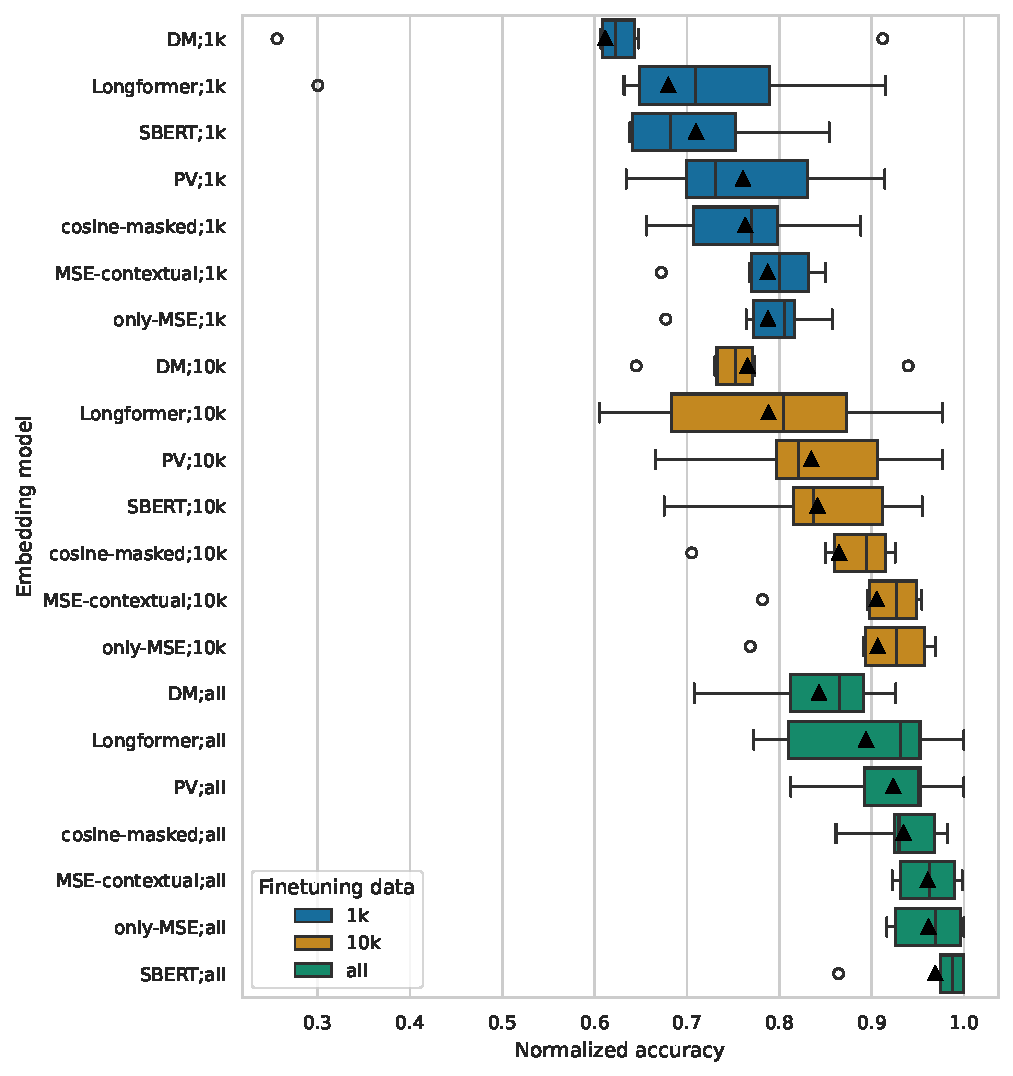
\includegraphics[width=\textwidth]{img/final_eval_norm_all.pdf}

  \caption{Overall relative performance of embedding models throughout the three
  rounds. In the first two rounds, we limit the number of finetuning documents to 1k
  and 10k, but do not set any limit in the third round labeled as ``all''.}

  \label{fig:final_eval_norm_all}

\end{figure}

In the first round, Longformer's and SBERT's performance is underwhelming. At
the same time, the best student model achieves, on average, nearly 80\% of the
best performance for a given task achieved by an embedding model with all
finetuning data. We see this as a considerable achievement since there are 17
to 240 times more finetuning documents in the last round compared to the first
one. In the second round, the classifiers are trained on 10k finetuning
documents, and their performances naturally increase. Particularly for SBERT, as
it now surpasses \Model{PV}, which improves by a relatively small amount. These
effects are also noticeable in the performance of {\CosineStudent} as there is
a more significant gap between it and the other two students that rely on
SBERT more. Finally, with all finetuning data, the differences between models'
performances diminish as the best models improve only marginally. SBERT takes
the greatest advantage of the increase in finetuning data and surpasses all
other models. We see this as a demonstration that the embedding model does not
strictly need a large maximum context for the selected set of tasks. In other
words, despite the moderately large documents, we can reach a competitive
performance by only considering the first 384 tokens of each input. This is
apparent, especially for \Task{arxiv}, where we can imagine classifying the
field of a scholarly paper based on just its abstract. So, as the context is of
minor importance, SBERT benefits from its full attention and surpasses the best
student by a small fraction. Nonetheless, all student models can improve the
scores of their contextual teachers and base checkpoints. Moreover, the
students reach consistent and comparable performances despite being trained
differently. {\CosineStudent} trains with a different contextual teacher,
contextual loss, structural loss, and weighting of the two losses than the rest
of the students. {\MSEStudent} trains with a significantly less performant
contextual teacher, while {\OnlyMSEStudent} does not use a contextual teacher.
This shows that our method is robust and open to multiple changes in various
aspects.

We now examine the models' performances per each task, which we plot in
Figure~\ref{fig:final_cls_evals}. The relative models' performances on a given
task stay consistent throughout the three rounds, so we focus only on the last
two. With 10k finetuning documents, the students perform best on
classifications of document pairs. On \Task{imdb}, Longformer shows the best
performance, which is surprising given it is the second-worst model in both
rounds. On \Task{arxiv}, PV shows the best performance as it benefits from its
large embedding and unlimited context. Arguably, both of these attributes play
a role, as \Model{DM} with the same unlimited context but with more than 50
times smaller embedding performs better than Longformer but worse than
\Model{PV}. As we increase the number of finetuning documents, SBERT
substantially improves. We register the largest performance increase for tasks
with the most finetuning data available. These are \Task{aan}, \Task{oc}, and
\Task{s2orc}. We also highlight SBERT's performance on \Task{arxiv} in both
rounds, where it outperforms all students with eight times larger maximum
context and comes relatively close to the performance of \Model{PV}. This
demonstrates that, despite the task being composed of only very long documents,
we can achieve a competitive performance based on just the first few hundred
tokens. The insignificance of an embedding model's lack of context may partly
explain why the students' performances for a given task are not affected by the
length of the tasks' documents. For example, on tasks with longer documents
such as \Task{arxiv} or \Task{pan}, {\CosineStudent} and {\MSEStudent} perform
on par with {\OnlyMSEStudent} despite being trained with a contextual teacher,
which should theoretically improve the students' performance on longer inputs.

\begin{figure}

  \centering
  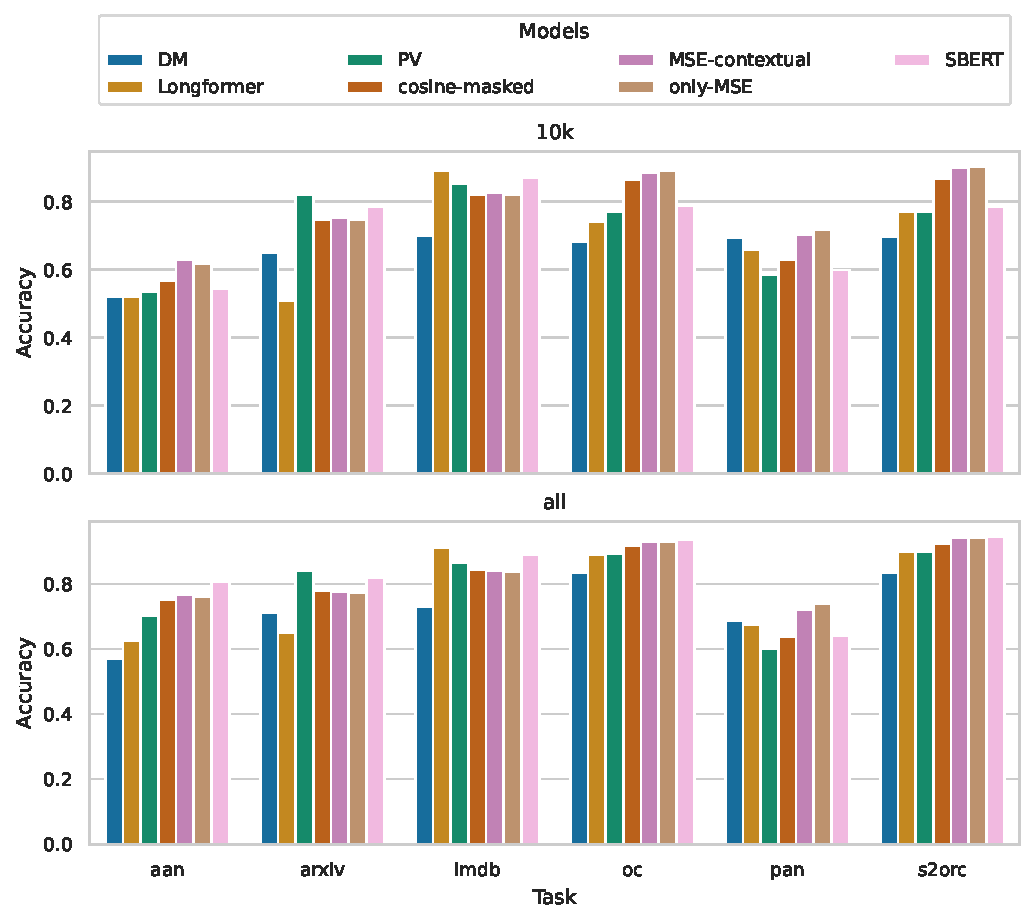
\includegraphics[width=\textwidth]{img/final_cls_evals.pdf}

  \caption{Performance of embedding models on evaluation tasks with the finetuning documents being limited to 10k and with all finetuning data.}

  \label{fig:final_cls_evals}

\end{figure}

\subsection{Retrieval tasks}

\begin{figure}[p]

  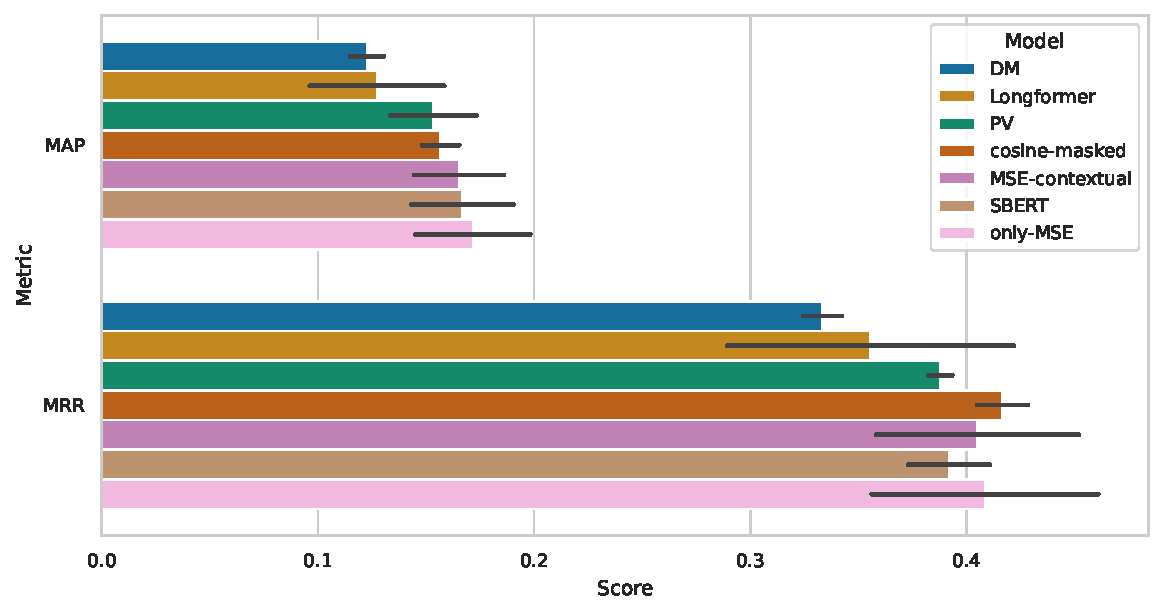
\includegraphics[width=\textwidth]{img/final_sims_evals.pdf}

  \caption{Performance of models on retrieval tasks. We mark the mean score
  with a bar and the span between each task's score with an error bar.}

  \label{fig:final_eval_sims}

\end{figure}

\begin{figure}[t]

  \centering
  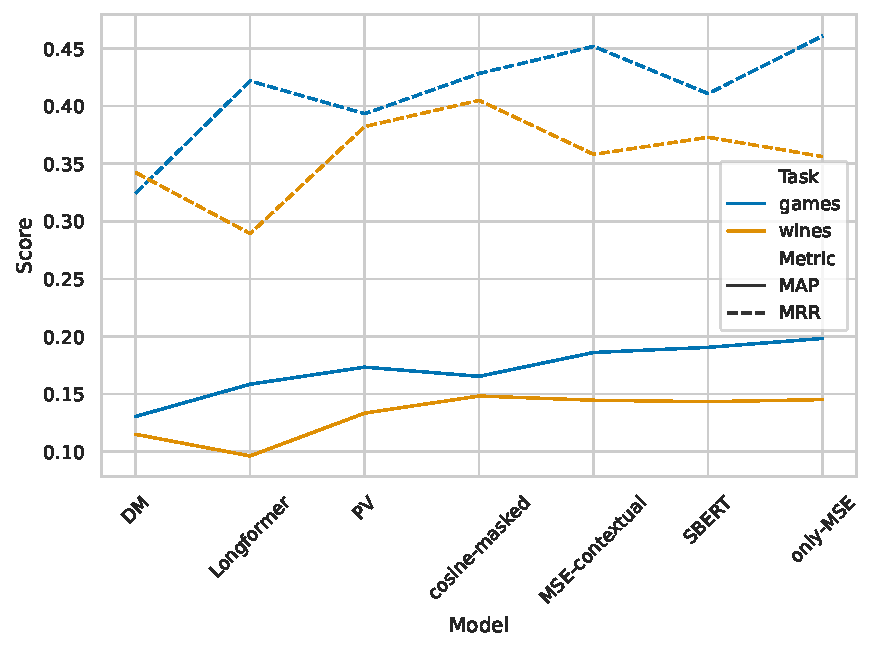
\includegraphics[width=0.85\textwidth]{img/final_sims_evals_per_task.pdf}

  \caption{Performance of embedding models on each retrieval task.}

  \label{fig:final_eval_sims_per_task}

\end{figure}

We plot the overall models' performances on the retrieval tasks in
Figure~\ref{fig:final_eval_sims}. In terms of MAP, the best-performing model is
{\OnlyMSEStudent} closely followed by SBERT and the other two student models.
For Mean Reciprocal Rank, the best model is {\CosineStudent}, one
of the most consistent models in both metrics. This suggests that using
a structural teacher only for inputs, which it can process as a whole, may lead to a
more consistent student model.


We also plot the models' performances per each task in
Figure~\ref{fig:final_eval_sims_per_task}. As the results suggest, \Task{games}
is an easier task than \Task{wines}. This may be unexpected since, compared to
\Task{wines}, \Task{games} has more total documents but a similar amount of
source and target documents. Consequently, \Task{games} contains much more
``noise'' documents, which may hurt the performance. However, as we mention in
the tasks' description, the selection of topics for \Task{games} is much wider,
and the differences between documents are far less nuanced. On the other hand,
the similarities of documents in \Task{wines} are sometimes based on a few
details mentioned throughout the document.

\chapter*{Conclusion}
\addcontentsline{toc}{chapter}{Conclusion}


%%% Bibliography
%%% Bibliography (literature used as a source)
%%%
%%% We employ bibTeX to construct the bibliography. It processes
%%% citations in the text (e.g., the \cite{...} macro) and looks up
%%% relevant entries in the bibliography.bib file.
%%%
%%% The \bibliographystyle command selects, which style will be used
%%% for references from the text. The argument in curly brackets is
%%% the name of the corresponding style file (*.bst). Both styles
%%% mentioned in this template are included in LaTeX distributions.

\bibliographystyle{plainnat}    %% Author (year)
% \bibliographystyle{unsrt}     %% [number]

\renewcommand{\bibname}{Bibliography}

%%% Generate the bibliography. Beware that if you cited no works,
%%% the empty list will be omitted completely.

\bibliography{bibliography}

\bigskip
\noindent
For final corrections we used Grammarly (\url{grammarly.com}).

%%% If case you prefer to write the bibliography manually (without bibTeX),
%%% you can use the following. Please follow the ISO 690 standard and
%%% citation conventions of your field of research.

% \begin{thebibliography}{99}
%
% \bibitem{lamport94}
%   {\sc Lamport,} Leslie.
%   \emph{\LaTeX: A Document Preparation System}.
%   2nd edition.
%   Massachusetts: Addison Wesley, 1994.
%   ISBN 0-201-52983-1.
%
% \end{thebibliography}


%%% Figures used in the thesis (consider if this is needed)
\listoffigures

%%% Tables used in the thesis (consider if this is needed)
%%% In mathematical theses, it could be better to move the list of tables to the beginning of the thesis.
\listoftables

%%% Abbreviations used in the thesis, if any, including their explanation
%%% In mathematical theses, it could be better to move the list of abbreviations to the beginning of the thesis.
% \chapwithtoc{List of Abbreviations}

%%% Attachments to the master thesis, if any. Each attachment must be
%%% referred to at least once from the text of the thesis. Attachments
%%% are numbered.
%%%
%%% The printed version should preferably contain attachments, which can be
%%% read (additional tables and charts, supplementary text, examples of
%%% program output, etc.). The electronic version is more suited for attachments
%%% which will likely be used in an electronic form rather than read (program
%%% source code, data files, interactive charts, etc.). Electronic attachments
%%% should be uploaded to SIS and optionally included in the thesis on a~CD/DVD.
%%% Allowed file formats are specified in the provision of the rector no. 72/2017.
\appendix
\chapter{Attachments}

% \section{First Attachment}

\openright
\end{document}
